\section{A Short C Reminder for Python Programmers}

\footnote{I would like to thank Gemini Pro for the contribution it has given to writing this wonderful section. Thank you bro, we've come a long way together.} Minimal understanding of C syntax is strictly needed for the upcoming topics of this course. Since many of you are coming from a pure Python background, this section will serve as a bridge. Python is incredibly flexible, dynamic, and high-level, but when raw performance and direct hardware manipulation are required, such as in GPU computing, C is the absolute standard.

\subsection{Compiled vs Interpreted Languages}

The most fundamental difference between Python and C is how the computer executes them. Python is an \textbf{interpreted} language. When you run a script, the Python interpreter reads and executes the code line by line on the fly, either through an interactive shell or by running a \texttt{.py} file. 

C, on the other hand, is a \textbf{compiled} language. Before you can run a C program, you must pass the source code through a compiler (like \texttt{gcc}, \texttt{g++}, or \texttt{cc} on Linux). The compiler translates your entire human-readable code into a machine-executable binary file. 

This additional step makes development slightly slower, but the resulting execution is exponentially faster. Moreover, while Python reveals syntax errors only when it tries to execute the flawed line, the C compiler will catch all syntax errors beforehand, completely preventing compilation until they are fixed.

Let's now take a look at a simple program in C and go through with its execution.

\subsection{The anatomy of a basic C program}

Here it is: the classic "Hello World" program. 

\begin{Verbatim}[label=\makebox{\url{https://github.com/lucabaldini/cmepda/tree/master/slides/latex/snippets/hello_world.c}},commandchars=\\\{\}]
\PY{c+cp}{\#}\PY{c+cp}{include}\PY{+w}{ }\PY{c+cpf}{\PYZlt{}stdio.h\PYZgt{}}

\PY{k+kt}{int}\PY{+w}{ }\PY{n+nf}{main}\PY{p}{(}\PY{p}{)}\PY{+w}{ }\PY{p}{\PYZob{}}
\PY{+w}{    }\PY{c+cm}{/* my first program in C */}
\PY{+w}{    }\PY{n}{printf}\PY{p}{(}\PY{l+s}{\PYZdq{}}\PY{l+s}{Hello World! }\PY{l+s+se}{\PYZbs{}n}\PY{l+s}{\PYZdq{}}\PY{p}{)}\PY{p}{;}

\PY{+w}{    }\PY{k}{return}\PY{+w}{ }\PY{l+m+mi}{0}\PY{p}{;}
\PY{p}{\PYZcb{}}

[Output]
Hello World! 
\end{Verbatim}

Now, let's analyse this piece of code step by step so we can start understanding the C syntax. 
\begin{itemize}
    \item First of all, you must know that in Python, code can simply exist in the global scope, but in C code to be executed \textit{must} be enclosed within "functions". As an absolute minimum, every program must have a function called \textbf{\texttt{main}} (line 3)
    \item Python uses indentation to define blocks of code. In C, \textbf{blocks} of code instructions are enclosed in braces \textbf{\texttt{\{ \}}} (lines 3 and 8) and indentation is purely for human readability.
    \item Every single instruction (\textbf{statement}) must end with a semicolon \textbf{\texttt{;}} (line 7). Forgetting this is the most common cause of compiler errors.
    \item Text \textbf{strings} are enclosed by double quotes \textbf{\texttt{" "}} (line 5). Single quotes \texttt{' '} are strictly used for single characters only.
    \item Multi-line \textbf{comments} are enclosed by \textbf{\texttt{/* ... */}} (line 4). Single-line comments use {\texttt{/ /}} instead.
    \item You can include other pieces of code with the \texttt{\#include} directive (line 1). The \texttt{\#include <stdio.h>} line tells the compiler to include the \textit{Standard Input/Output library}, which is necessary to use the \texttt{printf} function. More generally, the word that comes after the \textbf{\texttt{\#}} symbol is called a \textbf{directive}, and, roughly speaking, it constitutes an "order" to the compiler (this concept will become clearer later).
    \item The \texttt{return 0} instruction (line 7) is not mandatory, but you will always find it for good practice at the end of each C program.
\end{itemize}

Now let's say that you have opened your favourite text editor and written the example program above in a file called \texttt{hello\_world.c} (the \texttt{.c} part is necessary, otherwise your compiler won't recognize the file). Let's also say that the file is saved in the directory \texttt{c/introduction\_to\_C}. If you are using Linux (as you should), in order to compile your file you must open the terminal, move inside the directory and then type \texttt{gcc hello\_world.c} (the same would be true on Windows). This will create an executable named \texttt{a.out} (or \texttt{a.exe} on Windows). In order to give it a more meaningful name, use the \texttt{-o} flag, just like this: \texttt{gcc hello\_world.c -o hello\_world} (on Windows you should type \texttt{gcc hello\_world.c -o hello\_world.exe}). \\ Once compiled, to run your program on Linux type \texttt{./hello\_world}. The \texttt{./} is mandatory as it tells the OS to look for the executable in the current directory (on Windows, you can simply type \texttt{hello\_world.exe} or just \texttt{hello\_world}). \footnote{Once you've become familiar with this process, you should consider switching to VS Code, which can hide all this operations for you and let you run C code just like a Python script.}

\subsection{Identifiers, Types and Variables}

Variables and functions names in C are called \textbf{identifiers}. An identifier must start with a letter or an underscore (not a number), and can then contain letters, numbers, and underscores. 

\begin{center}
    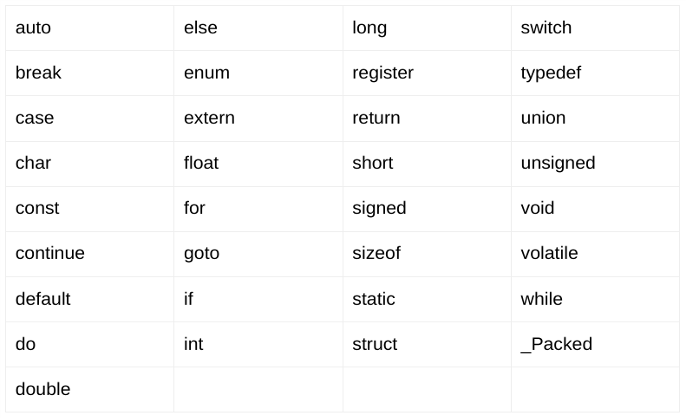
\includegraphics[width=0.65\textwidth]{figuresP/lesson_parallel_3a_pag_11.png}
\end{center}

Crucially, an identifier cannot be one of the reserved C \textbf{keywords} reported below.

\begin{center}
    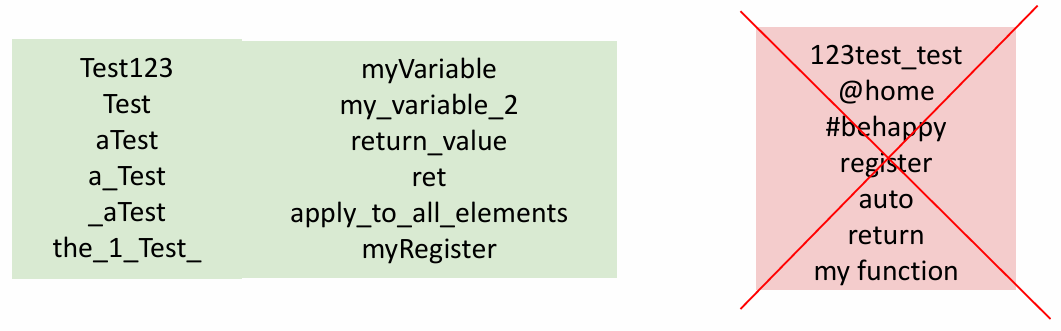
\includegraphics[width=0.65\textwidth]{figuresP/lesson_parallel_3a_pag_12.png}
\end{center}

Python is dynamically typed, while C is \textbf{statically typed}. That means that you must declare a variable type before using it through the syntax \texttt{type variablename;}. Here is a brief overview of the main variable types in C (you will find an example at the end of the list):

\subsubsection{- Integers and Floating Point numbers}

You can define integers and floating point numbers in many ways depending on your needs and your required precision, as shown in the following table.

\begin{table}[h]
\centering
\begin{tabular}{|c|c|c|c|}
\hline
\textbf{Type} & \textbf{Size (bits)} & \textbf{Size (bytes)} & \textbf{Range} \\
\hline
char & 8 & 1 & -128 to 127 \\
\hline
unsigned char & 8 & 1 & 0 to 255 \\
\hline
int & 16 & 2 & $-2^{15}$ to $2^{15}-1$ \\
\hline
unsigned int & 16 & 2 & 0 to $2^{16}-1$ \\
\hline
short int & 8 & 1 & -128 to 127 \\
\hline
unsigned short int & 8 & 1 & 0 to 255 \\
\hline
long int & 32 & 4 & $-2^{31}$ to $2^{31}-1$ \\
\hline
unsigned long int & 32 & 4 & 0 to $2^{32}-1$ \\
\hline
float & 32 & 4 & 3.4E-38 to 3.4E+38 \\
\hline
double & 64 & 8 & 1.7E-308 to 1.7E+308 \\
\hline
long double & 80 & 10 & 3.4E-4932 to 1.1E+4932 \\
\hline
\end{tabular}
\end{table}

Take a look at the different possible syntaxes for variable definition and printing methods in this example: 

\begin{Verbatim}[label=\makebox{\url{https://github.com/lucabaldini/cmepda/tree/master/slides/latex/snippets/variables_and_printf.c}},commandchars=\\\{\}]
\PY{c+cp}{\#}\PY{c+cp}{include}\PY{+w}{ }\PY{c+cpf}{\PYZlt{}stdio.h\PYZgt{}}
\PY{k+kt}{int}\PY{+w}{ }\PY{n+nf}{main}\PY{p}{(}\PY{p}{)}\PY{+w}{ }\PY{p}{\PYZob{}}
\PY{+w}{    }\PY{c+cm}{// Variable definition }
\PY{+w}{    }\PY{k+kt}{int}\PY{+w}{ }\PY{n}{a}\PY{p}{,}\PY{+w}{ }\PY{n}{b}\PY{p}{,}\PY{+w}{ }\PY{n}{c}\PY{p}{;}
\PY{+w}{    }\PY{n}{a}\PY{+w}{ }\PY{o}{=}\PY{+w}{ }\PY{l+m+mi}{2}\PY{p}{;}
\PY{+w}{    }\PY{n}{printf}\PY{p}{(}\PY{l+s}{\PYZdq{}}\PY{l+s}{a = \PYZpc{}d}\PY{l+s+se}{\PYZbs{}n}\PY{l+s}{\PYZdq{}}\PY{p}{,}\PY{+w}{ }\PY{n}{a}\PY{p}{)}\PY{p}{;}
\PY{+w}{    }\PY{k+kt}{int}\PY{+w}{ }\PY{n}{d}\PY{+w}{ }\PY{o}{=}\PY{+w}{ }\PY{l+m+mi}{1}\PY{p}{;}
\PY{+w}{    }\PY{k+kt}{float}\PY{+w}{ }\PY{n}{e}\PY{p}{;}
\PY{+w}{    }\PY{n}{e}\PY{+w}{ }\PY{o}{=}\PY{+w}{ }\PY{l+m+mf}{2.0}\PY{p}{;}
\PY{+w}{    }\PY{k+kt}{float}\PY{+w}{ }\PY{n}{f}\PY{+w}{ }\PY{o}{=}\PY{+w}{ }\PY{l+m+mf}{1.27}\PY{p}{;}
\PY{+w}{    }\PY{k+kt}{double}\PY{+w}{ }\PY{n}{g}\PY{+w}{ }\PY{o}{=}\PY{+w}{ }\PY{l+m+mf}{2.19293993847}\PY{p}{;}

\PY{+w}{    }\PY{n}{printf}\PY{p}{(}\PY{l+s}{\PYZdq{}}\PY{l+s}{e = \PYZpc{}d, }\PY{l+s}{\PYZdq{}}\PY{p}{,}\PY{+w}{ }\PY{n}{e}\PY{p}{)}\PY{p}{;}\PY{+w}{  }\PY{c+cm}{// Never pass a float and declare int !!!}
\PY{+w}{    }\PY{n}{printf}\PY{p}{(}\PY{l+s}{\PYZdq{}}\PY{l+s}{e = \PYZpc{}f, }\PY{l+s}{\PYZdq{}}\PY{p}{,}\PY{+w}{ }\PY{n}{e}\PY{p}{)}\PY{p}{;}
\PY{+w}{    }\PY{n}{printf}\PY{p}{(}\PY{l+s}{\PYZdq{}}\PY{l+s}{e = \PYZpc{}.1f}\PY{l+s+se}{\PYZbs{}n}\PY{l+s}{\PYZdq{}}\PY{p}{,}\PY{+w}{ }\PY{n}{e}\PY{p}{)}\PY{p}{;}

\PY{+w}{    }\PY{n}{printf}\PY{p}{(}\PY{l+s}{\PYZdq{}}\PY{l+s}{g = \PYZpc{}d, }\PY{l+s}{\PYZdq{}}\PY{p}{,}\PY{+w}{ }\PY{n}{g}\PY{p}{)}\PY{p}{;}\PY{+w}{  }\PY{c+cm}{// Never pass a float and declare int !!!}
\PY{+w}{    }\PY{n}{printf}\PY{p}{(}\PY{l+s}{\PYZdq{}}\PY{l+s}{g = \PYZpc{}f, }\PY{l+s}{\PYZdq{}}\PY{p}{,}\PY{+w}{ }\PY{n}{g}\PY{p}{)}\PY{p}{;}
\PY{+w}{    }\PY{n}{printf}\PY{p}{(}\PY{l+s}{\PYZdq{}}\PY{l+s}{g = \PYZpc{}.11f}\PY{l+s}{\PYZdq{}}\PY{p}{,}\PY{+w}{ }\PY{n}{g}\PY{p}{)}\PY{p}{;}

\PY{+w}{    }\PY{k}{return}\PY{+w}{ }\PY{l+m+mi}{0}\PY{p}{;}
\PY{p}{\PYZcb{}}

[Output]
a = 2
e = 0, e = 2.000000, e = 2.0
g = 405705013, g = 2.192940, g = 2.19293993847
\end{Verbatim}

\subsubsection{- Booleans}

Booleans are not defined in plain C. You must \texttt{\#include <stdbool.h>} to have the \texttt{bool} type defined. Otherwise, you can use the smallest integer (\texttt{char}) to represent them as 1 (true) and 0 (false).

\begin{Verbatim}[label=\makebox{\url{https://github.com/lucabaldini/cmepda/tree/master/slides/latex/snippets/booleans_in_c.c}},commandchars=\\\{\}]
\PY{c+cp}{\#}\PY{c+cp}{include}\PY{+w}{ }\PY{c+cpf}{\PYZlt{}stdio.h\PYZgt{}}
\PY{c+cp}{\#}\PY{c+cp}{include}\PY{+w}{ }\PY{c+cpf}{\PYZlt{}stdbool.h\PYZgt{}}\PY{c+c1}{ // Lets you use \PYZsq{}bool\PYZsq{}, \PYZsq{}true\PYZsq{} and \PYZsq{}false\PYZsq{}}

\PY{k+kt}{int}\PY{+w}{ }\PY{n+nf}{main}\PY{p}{(}\PY{p}{)}\PY{+w}{ }\PY{p}{\PYZob{}}
\PY{+w}{    }\PY{c+cm}{// Variable definition}
\PY{+w}{    }\PY{k+kt}{bool}\PY{+w}{ }\PY{n}{first\_method}\PY{+w}{ }\PY{o}{=}\PY{+w}{ }\PY{n+nb}{true}\PY{p}{;}
\PY{+w}{    }\PY{k+kt}{char}\PY{+w}{ }\PY{n}{second\_method}\PY{+w}{ }\PY{o}{=}\PY{+w}{ }\PY{l+m+mi}{1}\PY{p}{;}

\PY{+w}{    }\PY{n}{printf}\PY{p}{(}\PY{l+s}{\PYZdq{}}\PY{l+s}{bool (\PYZlt{}stdbool.h\PYZgt{}): \PYZpc{}d}\PY{l+s+se}{\PYZbs{}n}\PY{l+s}{\PYZdq{}}\PY{p}{,}\PY{+w}{ }\PY{n}{first\_method}\PY{p}{)}\PY{p}{;}
\PY{+w}{    }\PY{n}{printf}\PY{p}{(}\PY{l+s}{\PYZdq{}}\PY{l+s}{char (Plain C):     \PYZpc{}d}\PY{l+s+se}{\PYZbs{}n}\PY{l+s}{\PYZdq{}}\PY{p}{,}\PY{+w}{ }\PY{n}{second\_method}\PY{p}{)}\PY{p}{;}

\PY{+w}{    }\PY{k}{return}\PY{+w}{ }\PY{l+m+mi}{0}\PY{p}{;}
\PY{p}{\PYZcb{}}

[Output]
bool (<stdbool.h>): 1
char (Plain C):     1
\end{Verbatim}

\subsubsection{- Literals}

Constants or \textbf{literals} are fixed values explicitly defined in the code that cannot be modified during execution. In C, you can specify the exact type and base of a literal using specific prefixes and suffixes. This is particularly important because the compiler assigns default types to literals, which can affect the precision of mathematical operations.

\begin{itemize}
    \item[-] \textit{Integer literals:} They can be written in decimal, hexadecimal (using the \texttt{0x} prefix), or even octal format. You can append suffixes to specify their exact type: \texttt{U} or \texttt{u} for \texttt{unsigned}, and \texttt{L} or \texttt{l} for \texttt{long} (e.g., \texttt{1L}, \texttt{3U}).
    \item[-] \textit{Floating-point literals:} By default, any numerical literal with a decimal point is treated as a \texttt{double}. If you want to specify a \texttt{float}, you must append the \texttt{f} suffix (e.g., \texttt{1.f} or \texttt{3.14f}). For a \texttt{long double}, use the \texttt{L} suffix. You can also use \texttt{E} or \texttt{e} to indicate exponents in scientific notation.
\end{itemize}

Take a look at how different literal suffixes affect the precision and the result of a simple division in this example:

\begin{Verbatim}[label=\makebox{\url{https://github.com/lucabaldini/cmepda/tree/master/slides/latex/snippets/literals_and_precision.c}},commandchars=\\\{\}]
\PY{c+cp}{\#}\PY{c+cp}{include}\PY{+w}{ }\PY{c+cpf}{\PYZlt{}stdio.h\PYZgt{}}

\PY{k+kt}{int}\PY{+w}{ }\PY{n+nf}{main}\PY{p}{(}\PY{p}{)}\PY{+w}{ }\PY{p}{\PYZob{}}
\PY{+w}{    }\PY{c+c1}{// Integer Literals}
\PY{+w}{    }\PY{k+kt}{int}\PY{+w}{ }\PY{n}{dec}\PY{+w}{ }\PY{o}{=}\PY{+w}{ }\PY{l+m+mi}{42}\PY{p}{;}\PY{+w}{           }\PY{c+c1}{// Standard decimal}
\PY{+w}{    }\PY{k+kt}{int}\PY{+w}{ }\PY{n}{hex}\PY{+w}{ }\PY{o}{=}\PY{+w}{ }\PY{l+m+mh}{0x2A}\PY{p}{;}\PY{+w}{         }\PY{c+c1}{// Hexadecimal (0x prefix)}
\PY{+w}{    }\PY{k+kt}{int}\PY{+w}{ }\PY{n}{oct}\PY{+w}{ }\PY{o}{=}\PY{+w}{ }\PY{l+m+mo}{052}\PY{p}{;}\PY{+w}{          }\PY{c+c1}{// Octal (0 prefix)}
\PY{+w}{    }\PY{k+kt}{unsigned}\PY{+w}{ }\PY{k+kt}{int}\PY{+w}{ }\PY{n}{u}\PY{+w}{ }\PY{o}{=}\PY{+w}{ }\PY{l+m+mi}{42U}\PY{p}{;}\PY{+w}{   }\PY{c+c1}{// Unsigned (U or u suffix)}
\PY{+w}{    }\PY{k+kt}{long}\PY{+w}{ }\PY{k+kt}{int}\PY{+w}{ }\PY{n}{l}\PY{+w}{ }\PY{o}{=}\PY{+w}{ }\PY{l+m+mf}{42L}\PY{p}{;}\PY{+w}{       }\PY{c+c1}{// Long (L or l suffix)}

\PY{+w}{    }\PY{c+c1}{// Floating\PYZhy{}point Literals}
\PY{+w}{    }\PY{k+kt}{double}\PY{+w}{ }\PY{n}{d}\PY{+w}{ }\PY{o}{=}\PY{+w}{ }\PY{l+m+mf}{3.14}\PY{p}{;}\PY{+w}{        }\PY{c+c1}{// Double (Default)}
\PY{+w}{    }\PY{k+kt}{float}\PY{+w}{ }\PY{n}{f}\PY{+w}{ }\PY{o}{=}\PY{+w}{ }\PY{l+m+mf}{3.14f}\PY{p}{;}\PY{+w}{        }\PY{c+c1}{// Float (f or F suffix)}
\PY{+w}{    }\PY{k+kt}{long}\PY{+w}{ }\PY{k+kt}{double}\PY{+w}{ }\PY{n}{ld}\PY{+w}{ }\PY{o}{=}\PY{+w}{ }\PY{l+m+mf}{3.14L}\PY{p}{;}\PY{+w}{ }\PY{c+c1}{// Long double (L suffix)}
\PY{+w}{    }\PY{k+kt}{double}\PY{+w}{ }\PY{n}{sci}\PY{+w}{ }\PY{o}{=}\PY{+w}{ }\PY{l+m+mf}{3.14e\PYZhy{}2}\PY{p}{;}\PY{+w}{   }\PY{c+c1}{// Scientific notation (e or E exponent)}

\PY{+w}{    }\PY{c+c1}{// Precision Division Example}
\PY{+w}{    }\PY{c+c1}{// Demonstration of how suffixes affect the calculation}
\PY{+w}{    }\PY{k+kt}{long}\PY{+w}{ }\PY{k+kt}{double}\PY{+w}{ }\PY{n}{r}\PY{p}{;}

\PY{+w}{    }\PY{n}{r}\PY{+w}{ }\PY{o}{=}\PY{+w}{ }\PY{l+m+mi}{1}\PY{+w}{ }\PY{o}{/}\PY{+w}{ }\PY{l+m+mi}{3}\PY{p}{;}
\PY{+w}{    }\PY{n}{printf}\PY{p}{(}\PY{l+s}{\PYZdq{}}\PY{l+s}{1/3     (int)         = \PYZpc{}.30Lf}\PY{l+s+se}{\PYZbs{}n}\PY{l+s}{\PYZdq{}}\PY{p}{,}\PY{+w}{ }\PY{n}{r}\PY{p}{)}\PY{p}{;}
\PY{+w}{    }\PY{n}{r}\PY{+w}{ }\PY{o}{=}\PY{+w}{ }\PY{l+m+mf}{1.f}\PY{+w}{ }\PY{o}{/}\PY{+w}{ }\PY{l+m+mf}{3.f}\PY{p}{;}
\PY{+w}{    }\PY{n}{printf}\PY{p}{(}\PY{l+s}{\PYZdq{}}\PY{l+s}{1.f/3.f (float)       = \PYZpc{}.30Lf}\PY{l+s+se}{\PYZbs{}n}\PY{l+s}{\PYZdq{}}\PY{p}{,}\PY{+w}{ }\PY{n}{r}\PY{p}{)}\PY{p}{;}
\PY{+w}{    }\PY{n}{r}\PY{+w}{ }\PY{o}{=}\PY{+w}{ }\PY{l+m+mf}{1.}\PY{+w}{ }\PY{o}{/}\PY{+w}{ }\PY{l+m+mf}{3.}\PY{p}{;}
\PY{+w}{    }\PY{n}{printf}\PY{p}{(}\PY{l+s}{\PYZdq{}}\PY{l+s}{1./3.   (double)      = \PYZpc{}.30Lf}\PY{l+s+se}{\PYZbs{}n}\PY{l+s}{\PYZdq{}}\PY{p}{,}\PY{+w}{ }\PY{n}{r}\PY{p}{)}\PY{p}{;}
\PY{+w}{    }\PY{n}{r}\PY{+w}{ }\PY{o}{=}\PY{+w}{ }\PY{l+m+mf}{1.L}\PY{+w}{ }\PY{o}{/}\PY{+w}{ }\PY{l+m+mf}{3.L}\PY{p}{;}
\PY{+w}{    }\PY{n}{printf}\PY{p}{(}\PY{l+s}{\PYZdq{}}\PY{l+s}{1.L/3.L (long double) = \PYZpc{}.30Lf}\PY{l+s+se}{\PYZbs{}n}\PY{l+s}{\PYZdq{}}\PY{p}{,}\PY{+w}{ }\PY{n}{r}\PY{p}{)}\PY{p}{;}
\PY{+w}{    }\PY{n}{r}\PY{+w}{ }\PY{o}{=}\PY{+w}{ }\PY{l+m+mf}{1L}\PY{+w}{ }\PY{o}{/}\PY{+w}{ }\PY{l+m+mf}{3L}\PY{p}{;}
\PY{+w}{    }\PY{n}{printf}\PY{p}{(}\PY{l+s}{\PYZdq{}}\PY{l+s}{1L/3L   (long int)    = \PYZpc{}.30Lf}\PY{l+s+se}{\PYZbs{}n}\PY{l+s}{\PYZdq{}}\PY{p}{,}\PY{+w}{ }\PY{n}{r}\PY{p}{)}\PY{p}{;}
\PY{+w}{    }\PY{k}{return}\PY{+w}{ }\PY{l+m+mi}{0}\PY{p}{;}
\PY{p}{\PYZcb{}}

[Output]
1/3     (int)         = 0.000000000000000000000000000000
1.f/3.f (float)       = 0.333333343267440795898437500000
1./3.   (double)      = 0.333333333333333314829616256247
1.L/3.L (long double) = 0.333333333333333333342368351437
1L/3L   (long int)    = 0.000000000000000000000000000000
\end{Verbatim}

\hrulefill

\subsubsection{Note: Variables vs. Literals} 
The variables defined in the latter piece of code seem very similar to what we have seen in the paragraph about "Integers and Floating Point numbers", don't they? \\
It is essential to distinguish between variables and literals, which represent the container and the content, respectively. While data types (e.g., \texttt{int}, \texttt{float}) define the size and range of the memory \textit{containers} used to store data, literals are the raw, immutable \textit{values} written directly into the source code. For instance, in the statement \texttt{float f = 3.14f;}, \texttt{float f} allocates a 32-bit variable (the container), whereas \texttt{3.14f} is a float literal specifying that the hardcoded value must be interpreted explicitly as a float rather than the default double (the content).\\
That distinction must be perfectly clear!

\hrulefill

\subsection{Operators}

Now that you know how to declare variables, it is time to manipulate them. \textbf{Operators} in C share many similarities with Python, but there are a few fundamental distinctions, particularly concerning how true/false evaluations and bit-level operations are handled. Take a look at the examples after each paragraph to better understand these peculiarities. 

\subsubsection{- Math and Relational Operators}

Math operators in C implement standard arithmetic operations. Most of them are binary (e.g., \texttt{a + b}, \texttt{a * b}, \texttt{a \% b} for the modulo), but unary operators exist as well, such as the minus sign to negate a variable (\texttt{-a}).

Relational operators are used to compare two variables and are practically equivalent to their Python counterparts: \texttt{>}, \texttt{<}, \texttt{>=}, \texttt{<=}, \texttt{!=}, and \texttt{==}. Note that the operator to check if two variables have the same value is \texttt{==}, which must never be confused with the assignment operator \texttt{=}.

Since C originally lacked a native boolean type, relational operators return \texttt{1} for true and \texttt{0} for false. Furthermore, the unary logical NOT operator \texttt{!} considers \texttt{0} as false and any non-zero value as true. Consequently, negating a true value like 10 (\texttt{!10}) yields \texttt{0} (false). 

\begin{Verbatim}[label=\makebox{\url{https://github.com/lucabaldini/cmepda/tree/master/slides/latex/snippets/operators.c}},commandchars=\\\{\}]
\PY{c+cp}{\#}\PY{c+cp}{include}\PY{+w}{ }\PY{c+cpf}{\PYZlt{}stdio.h\PYZgt{}}
\PY{k+kt}{int}\PY{+w}{ }\PY{n+nf}{main}\PY{p}{(}\PY{p}{)}\PY{+w}{ }\PY{p}{\PYZob{}}
\PY{+w}{    }\PY{k+kt}{int}\PY{+w}{ }\PY{n}{a}\PY{+w}{ }\PY{o}{=}\PY{+w}{ }\PY{l+m+mi}{10}\PY{p}{;}
\PY{+w}{    }\PY{k+kt}{int}\PY{+w}{ }\PY{n}{b}\PY{+w}{ }\PY{o}{=}\PY{+w}{ }\PY{l+m+mi}{7}\PY{p}{;}

\PY{+w}{    }\PY{c+c1}{// Math operators}
\PY{+w}{    }\PY{n}{printf}\PY{p}{(}\PY{l+s}{\PYZdq{}}\PY{l+s}{a+b=\PYZpc{}d}\PY{l+s+se}{\PYZbs{}n}\PY{l+s}{\PYZdq{}}\PY{p}{,}\PY{+w}{ }\PY{n}{a}\PY{o}{+}\PY{n}{b}\PY{p}{)}\PY{p}{;}\PY{+w}{    }\PY{c+c1}{// a+b=17}
\PY{+w}{    }\PY{n}{printf}\PY{p}{(}\PY{l+s}{\PYZdq{}}\PY{l+s}{a\PYZhy{}b=\PYZpc{}d}\PY{l+s+se}{\PYZbs{}n}\PY{l+s}{\PYZdq{}}\PY{p}{,}\PY{+w}{ }\PY{n}{a}\PY{o}{\PYZhy{}}\PY{n}{b}\PY{p}{)}\PY{p}{;}\PY{+w}{    }\PY{c+c1}{// a\PYZhy{}b=3}
\PY{+w}{    }\PY{n}{printf}\PY{p}{(}\PY{l+s}{\PYZdq{}}\PY{l+s}{a*b=\PYZpc{}d}\PY{l+s+se}{\PYZbs{}n}\PY{l+s}{\PYZdq{}}\PY{p}{,}\PY{+w}{ }\PY{n}{a}\PY{o}{*}\PY{n}{b}\PY{p}{)}\PY{p}{;}\PY{+w}{    }\PY{c+c1}{// a*b=70}
\PY{+w}{    }\PY{n}{printf}\PY{p}{(}\PY{l+s}{\PYZdq{}}\PY{l+s}{a/b=\PYZpc{}d}\PY{l+s+se}{\PYZbs{}n}\PY{l+s}{\PYZdq{}}\PY{p}{,}\PY{+w}{ }\PY{n}{a}\PY{o}{/}\PY{n}{b}\PY{p}{)}\PY{p}{;}\PY{+w}{    }\PY{c+c1}{// a/b=1 (integer division!)}
\PY{+w}{    }\PY{n}{printf}\PY{p}{(}\PY{l+s}{\PYZdq{}}\PY{l+s}{a\PYZpc{}\PYZpc{}b=\PYZpc{}d}\PY{l+s+se}{\PYZbs{}n}\PY{l+s}{\PYZdq{}}\PY{p}{,}\PY{+w}{ }\PY{n}{a}\PY{o}{\PYZpc{}}\PY{n}{b}\PY{p}{)}\PY{p}{;}\PY{+w}{   }\PY{c+c1}{// a\PYZpc{}b=3}
\PY{+w}{    }\PY{n}{printf}\PY{p}{(}\PY{l+s}{\PYZdq{}}\PY{l+s}{\PYZhy{}a=\PYZpc{}d}\PY{l+s+se}{\PYZbs{}n}\PY{l+s}{\PYZdq{}}\PY{p}{,}\PY{+w}{ }\PY{o}{\PYZhy{}}\PY{n}{a}\PY{p}{)}\PY{p}{;}\PY{+w}{      }\PY{c+c1}{// \PYZhy{}a=\PYZhy{}10}
\PY{+w}{    }\PY{n}{printf}\PY{p}{(}\PY{l+s}{\PYZdq{}}\PY{l+s}{!a=\PYZpc{}d}\PY{l+s+se}{\PYZbs{}n}\PY{l+s}{\PYZdq{}}\PY{p}{,}\PY{+w}{ }\PY{o}{!}\PY{n}{a}\PY{p}{)}\PY{p}{;}\PY{+w}{      }\PY{c+c1}{// !a=0 (10 is true, so NOT 10 is false/0)}

\PY{+w}{    }\PY{c+c1}{// Relational operators}
\PY{+w}{    }\PY{n}{printf}\PY{p}{(}\PY{l+s}{\PYZdq{}}\PY{l+s}{a==b \PYZpc{}d}\PY{l+s+se}{\PYZbs{}n}\PY{l+s}{\PYZdq{}}\PY{p}{,}\PY{+w}{ }\PY{n}{a}\PY{o}{=}\PY{o}{=}\PY{n}{b}\PY{p}{)}\PY{p}{;}\PY{+w}{  }\PY{c+c1}{// a==b 0}
\PY{+w}{    }\PY{n}{printf}\PY{p}{(}\PY{l+s}{\PYZdq{}}\PY{l+s}{a!=b \PYZpc{}d}\PY{l+s+se}{\PYZbs{}n}\PY{l+s}{\PYZdq{}}\PY{p}{,}\PY{+w}{ }\PY{n}{a}\PY{o}{!}\PY{o}{=}\PY{n}{b}\PY{p}{)}\PY{p}{;}\PY{+w}{  }\PY{c+c1}{// a!=b 1}
\PY{+w}{    }\PY{n}{printf}\PY{p}{(}\PY{l+s}{\PYZdq{}}\PY{l+s}{a\PYZgt{}b  \PYZpc{}d}\PY{l+s+se}{\PYZbs{}n}\PY{l+s}{\PYZdq{}}\PY{p}{,}\PY{+w}{ }\PY{n}{a}\PY{o}{\PYZgt{}}\PY{n}{b}\PY{p}{)}\PY{p}{;}\PY{+w}{   }\PY{c+c1}{// a\PYZgt{}b 1}
\PY{+w}{    }\PY{n}{printf}\PY{p}{(}\PY{l+s}{\PYZdq{}}\PY{l+s}{a\PYZgt{}=b \PYZpc{}d}\PY{l+s+se}{\PYZbs{}n}\PY{l+s}{\PYZdq{}}\PY{p}{,}\PY{+w}{ }\PY{n}{a}\PY{o}{\PYZgt{}}\PY{o}{=}\PY{n}{b}\PY{p}{)}\PY{p}{;}\PY{+w}{  }\PY{c+c1}{// a\PYZgt{}=b 1}
\PY{+w}{    }\PY{n}{printf}\PY{p}{(}\PY{l+s}{\PYZdq{}}\PY{l+s}{a\PYZlt{}b  \PYZpc{}d}\PY{l+s+se}{\PYZbs{}n}\PY{l+s}{\PYZdq{}}\PY{p}{,}\PY{+w}{ }\PY{n}{a}\PY{o}{\PYZlt{}}\PY{n}{b}\PY{p}{)}\PY{p}{;}\PY{+w}{   }\PY{c+c1}{// a\PYZlt{}b 0}
\PY{+w}{    }\PY{n}{printf}\PY{p}{(}\PY{l+s}{\PYZdq{}}\PY{l+s}{a\PYZlt{}=b \PYZpc{}d}\PY{l+s+se}{\PYZbs{}n}\PY{l+s}{\PYZdq{}}\PY{p}{,}\PY{+w}{ }\PY{n}{a}\PY{o}{\PYZlt{}}\PY{o}{=}\PY{n}{b}\PY{p}{)}\PY{p}{;}\PY{+w}{  }\PY{c+c1}{// a\PYZlt{}=b 0}

\PY{+w}{    }\PY{k}{return}\PY{+w}{ }\PY{l+m+mi}{0}\PY{p}{;}
\PY{p}{\PYZcb{}}

[Output]
a+b=17
a-b=3
a*b=70
a/b=1
a%b=3
-a=-10
!a=0
a==b 0
a!=b 1
a>b  1
a>=b 1
a<b  0
a<=b 0
\end{Verbatim}

\subsubsection{- Logical vs Bitwise Operators}

In Python, you are used to writing \texttt{and}, \texttt{or}, and \texttt{not}. C introduces a strict separation between logical operations (which evaluate the overall truth of an expression) and bitwise operations (which act on the individual binary bits of the variables).

\begin{itemize}
    \item \textbf{Logical operators:} \texttt{\&\&} (AND), \texttt{||} (OR), and \texttt{!} (NOT). Just like in Python, they employ short-circuit evaluation: for example, the second operand in an OR expression is evaluated ONLY if the first one is false. They always return \texttt{0} or \texttt{1}.
    \item \textbf{Bitwise operators:} \texttt{\&} (AND), \texttt{|} (OR), \texttt{\^} (XOR), and \texttt{\~{}} (NOT). These act bit by bit. There are also the \texttt{>>} and \texttt{<<} operators, which shift the bits to the right or to the left, respectively.
\end{itemize}

\begin{Verbatim}[label=\makebox{\url{https://github.com/lucabaldini/cmepda/tree/master/slides/latex/snippets/bitwise_and_logical.c}},commandchars=\\\{\}]
\PY{c+cp}{\#}\PY{c+cp}{include}\PY{+w}{ }\PY{c+cpf}{\PYZlt{}stdio.h\PYZgt{}}

\PY{k+kt}{int}\PY{+w}{ }\PY{n+nf}{main}\PY{p}{(}\PY{p}{)}\PY{+w}{ }\PY{p}{\PYZob{}}
\PY{+w}{    }\PY{k+kt}{int}\PY{+w}{ }\PY{n}{a}\PY{+w}{ }\PY{o}{=}\PY{+w}{ }\PY{l+m+mi}{10}\PY{p}{;}\PY{+w}{  }\PY{c+c1}{// in binary: 00001010}
\PY{+w}{    }\PY{k+kt}{int}\PY{+w}{ }\PY{n}{b}\PY{+w}{ }\PY{o}{=}\PY{+w}{ }\PY{l+m+mi}{7}\PY{p}{;}\PY{+w}{   }\PY{c+c1}{// in binary: 00000111}

\PY{+w}{    }\PY{c+c1}{// Logical operators}
\PY{+w}{    }\PY{n}{printf}\PY{p}{(}\PY{l+s}{\PYZdq{}}\PY{l+s}{a \PYZam{}\PYZam{} b =\PYZgt{} \PYZpc{}d}\PY{l+s+se}{\PYZbs{}n}\PY{l+s}{\PYZdq{}}\PY{p}{,}\PY{+w}{ }\PY{n}{a}\PY{+w}{ }\PY{o}{\PYZam{}}\PY{o}{\PYZam{}}\PY{+w}{ }\PY{n}{b}\PY{p}{)}\PY{p}{;}\PY{+w}{ }\PY{c+c1}{// a AND b =\PYZgt{} 1}
\PY{+w}{    }\PY{n}{printf}\PY{p}{(}\PY{l+s}{\PYZdq{}}\PY{l+s}{a || b =\PYZgt{} \PYZpc{}d}\PY{l+s+se}{\PYZbs{}n}\PY{l+s}{\PYZdq{}}\PY{p}{,}\PY{+w}{ }\PY{n}{a}\PY{+w}{ }\PY{o}{|}\PY{o}{|}\PY{+w}{ }\PY{n}{b}\PY{p}{)}\PY{p}{;}\PY{+w}{ }\PY{c+c1}{// a OR b  =\PYZgt{} 1}
\PY{+w}{    }\PY{n}{printf}\PY{p}{(}\PY{l+s}{\PYZdq{}}\PY{l+s}{!a     =\PYZgt{} \PYZpc{}d}\PY{l+s+se}{\PYZbs{}n}\PY{l+s}{\PYZdq{}}\PY{p}{,}\PY{+w}{ }\PY{o}{!}\PY{n}{a}\PY{p}{)}\PY{p}{;}\PY{+w}{     }\PY{c+c1}{// NOT a   =\PYZgt{} 0}

\PY{+w}{    }\PY{c+c1}{// Bitwise operators}
\PY{+w}{    }\PY{n}{printf}\PY{p}{(}\PY{l+s}{\PYZdq{}}\PY{l+s}{a \PYZam{} b = \PYZpc{}d}\PY{l+s+se}{\PYZbs{}n}\PY{l+s}{\PYZdq{}}\PY{p}{,}\PY{+w}{ }\PY{n}{a}\PY{+w}{ }\PY{o}{\PYZam{}}\PY{+w}{ }\PY{n}{b}\PY{p}{)}\PY{p}{;}\PY{+w}{    }\PY{c+c1}{// 2    (00000010)}
\PY{+w}{    }\PY{n}{printf}\PY{p}{(}\PY{l+s}{\PYZdq{}}\PY{l+s}{a | b = \PYZpc{}d}\PY{l+s+se}{\PYZbs{}n}\PY{l+s}{\PYZdq{}}\PY{p}{,}\PY{+w}{ }\PY{n}{a}\PY{+w}{ }\PY{o}{|}\PY{+w}{ }\PY{n}{b}\PY{p}{)}\PY{p}{;}\PY{+w}{    }\PY{c+c1}{// 15   (00001111)}
\PY{+w}{    }\PY{n}{printf}\PY{p}{(}\PY{l+s}{\PYZdq{}}\PY{l+s}{a \PYZca{} b = \PYZpc{}d}\PY{l+s+se}{\PYZbs{}n}\PY{l+s}{\PYZdq{}}\PY{p}{,}\PY{+w}{ }\PY{n}{a}\PY{+w}{ }\PY{o}{\PYZca{}}\PY{+w}{ }\PY{n}{b}\PY{p}{)}\PY{p}{;}\PY{+w}{    }\PY{c+c1}{// 13   (00001101)}
\PY{+w}{    }\PY{n}{printf}\PY{p}{(}\PY{l+s}{\PYZdq{}}\PY{l+s}{\PYZti{}a    = \PYZpc{}d}\PY{l+s+se}{\PYZbs{}n}\PY{l+s}{\PYZdq{}}\PY{p}{,}\PY{+w}{ }\PY{o}{\PYZti{}}\PY{n}{a}\PY{p}{)}\PY{p}{;}\PY{+w}{       }\PY{c+c1}{// \PYZhy{}11  (11111111111111111111111111110101)}
\PY{+w}{    }\PY{n}{printf}\PY{p}{(}\PY{l+s}{\PYZdq{}}\PY{l+s}{a \PYZlt{}\PYZlt{} b = \PYZpc{}d}\PY{l+s+se}{\PYZbs{}n}\PY{l+s}{\PYZdq{}}\PY{p}{,}\PY{+w}{ }\PY{n}{a}\PY{+w}{ }\PY{o}{\PYZlt{}}\PY{o}{\PYZlt{}}\PY{+w}{ }\PY{n}{b}\PY{p}{)}\PY{p}{;}\PY{+w}{  }\PY{c+c1}{// 1280 (10100000000)}
\PY{+w}{    }\PY{n}{printf}\PY{p}{(}\PY{l+s}{\PYZdq{}}\PY{l+s}{a \PYZgt{}\PYZgt{} 1 = \PYZpc{}d}\PY{l+s+se}{\PYZbs{}n}\PY{l+s}{\PYZdq{}}\PY{p}{,}\PY{+w}{ }\PY{n}{a}\PY{+w}{ }\PY{o}{\PYZgt{}}\PY{o}{\PYZgt{}}\PY{+w}{ }\PY{l+m+mi}{1}\PY{p}{)}\PY{p}{;}\PY{+w}{  }\PY{c+c1}{// 5    (00000101)}

\PY{+w}{    }\PY{k}{return}\PY{+w}{ }\PY{l+m+mi}{0}\PY{p}{;}
\PY{p}{\PYZcb{}}

[Output]
a && b => 1
a || b => 1
!a     => 0
a & b = 2
a | b = 15
a ^ b = 13
~a    = -11
a << b = 1280
a >> 1 = 5
\end{Verbatim}

\subsubsection{- Assignment and Increment/Decrement Operators}

The assignment operator \texttt{=} changes the value of a variable. A peculiar feature of C is that the assignment operation itself returns the assigned value. For instance, the expression \texttt{c = (a = 3)} is perfectly valid and results in both \texttt{a} and \texttt{c} holding the value \texttt{3}.
Assignments can also be composed with binary operators (\texttt{+=}, \texttt{-=}, \texttt{>>=}, etc.), just like in Python.

A major novelty for Python programmers is the introduction of the increment (\texttt{++}) and decrement (\texttt{--}) operators. Their behavior changes drastically depending on their position relative to the variable:
\begin{itemize}
    \item \textbf{Postfixed} (e.g., \texttt{a++}): Returns the original value, then increments the variable.
    \item \textbf{Prefixed} (e.g., \texttt{++a}): Increments the variable first, then returns the new incremented value.
\end{itemize}

\begin{Verbatim}[label=\makebox{\url{https://github.com/lucabaldini/cmepda/tree/master/slides/latex/snippets/assignment_and_increment.c}},commandchars=\\\{\}]
\PY{c+cp}{\#}\PY{c+cp}{include}\PY{+w}{ }\PY{c+cpf}{\PYZlt{}stdio.h\PYZgt{}}

\PY{k+kt}{int}\PY{+w}{ }\PY{n+nf}{main}\PY{p}{(}\PY{p}{)}\PY{+w}{ }\PY{p}{\PYZob{}}
\PY{+w}{    }\PY{k+kt}{int}\PY{+w}{ }\PY{n}{a}\PY{+w}{ }\PY{o}{=}\PY{+w}{ }\PY{l+m+mi}{0}\PY{p}{;}
\PY{+w}{    }\PY{k+kt}{int}\PY{+w}{ }\PY{n}{b}\PY{+w}{ }\PY{o}{=}\PY{+w}{ }\PY{l+m+mi}{10}\PY{p}{;}

\PY{+w}{    }\PY{c+c1}{// Assignment operator}
\PY{+w}{    }\PY{n}{printf}\PY{p}{(}\PY{l+s}{\PYZdq{}}\PY{l+s}{\PYZpc{}d}\PY{l+s+se}{\PYZbs{}n}\PY{l+s}{\PYZdq{}}\PY{p}{,}\PY{+w}{ }\PY{n}{a}\PY{o}{=}\PY{n}{b}\PY{p}{)}\PY{p}{;}\PY{+w}{     }\PY{c+c1}{// 10 (assignment returns the assigned value)}
\PY{+w}{    }\PY{n}{printf}\PY{p}{(}\PY{l+s}{\PYZdq{}}\PY{l+s}{\PYZpc{}d}\PY{l+s+se}{\PYZbs{}n}\PY{l+s}{\PYZdq{}}\PY{p}{,}\PY{+w}{ }\PY{n}{b}\PY{o}{=}\PY{l+m+mi}{7}\PY{p}{)}\PY{p}{;}\PY{+w}{     }\PY{c+c1}{// 7}

\PY{+w}{    }\PY{c+c1}{// Composed assignment}
\PY{+w}{    }\PY{n}{a}\PY{+w}{ }\PY{o}{+}\PY{o}{=}\PY{+w}{ }\PY{n}{b}\PY{p}{;}\PY{+w}{                  }\PY{c+c1}{// a = a + b}
\PY{+w}{    }\PY{n}{printf}\PY{p}{(}\PY{l+s}{\PYZdq{}}\PY{l+s}{a+=b =\PYZgt{} \PYZpc{}d}\PY{l+s+se}{\PYZbs{}n}\PY{l+s}{\PYZdq{}}\PY{p}{,}\PY{+w}{ }\PY{n}{a}\PY{p}{)}\PY{p}{;}\PY{+w}{ }\PY{c+c1}{// 17}
\PY{+w}{    }\PY{n}{a}\PY{+w}{ }\PY{o}{\PYZhy{}}\PY{o}{=}\PY{+w}{ }\PY{n}{b}\PY{p}{;}\PY{+w}{                  }\PY{c+c1}{// a = a \PYZhy{} b}
\PY{+w}{    }\PY{n}{printf}\PY{p}{(}\PY{l+s}{\PYZdq{}}\PY{l+s}{a\PYZhy{}=b =\PYZgt{} \PYZpc{}d}\PY{l+s+se}{\PYZbs{}n}\PY{l+s}{\PYZdq{}}\PY{p}{,}\PY{+w}{ }\PY{n}{a}\PY{p}{)}\PY{p}{;}\PY{+w}{ }\PY{c+c1}{// 10}
\PY{+w}{    }\PY{n}{a}\PY{+w}{ }\PY{o}{\PYZgt{}}\PY{o}{\PYZgt{}}\PY{o}{=}\PY{+w}{ }\PY{l+m+mi}{2}\PY{p}{;}\PY{+w}{                 }\PY{c+c1}{// a = a \PYZgt{}\PYZgt{} 2}
\PY{+w}{    }\PY{n}{printf}\PY{p}{(}\PY{l+s}{\PYZdq{}}\PY{l+s}{a\PYZgt{}\PYZgt{}=2 =\PYZgt{} \PYZpc{}d}\PY{l+s+se}{\PYZbs{}n}\PY{l+s}{\PYZdq{}}\PY{p}{,}\PY{+w}{ }\PY{n}{a}\PY{p}{)}\PY{p}{;}\PY{+w}{ }\PY{c+c1}{// 2}

\PY{+w}{    }\PY{c+c1}{// Increment/Decrement operators}
\PY{+w}{    }\PY{n}{a}\PY{+w}{ }\PY{o}{=}\PY{+w}{ }\PY{l+m+mi}{10}\PY{p}{;}\PY{+w}{                  }\PY{c+c1}{// Resetting \PYZsq{}a\PYZsq{} to 10 for the next examples}

\PY{+w}{    }\PY{n}{printf}\PY{p}{(}\PY{l+s}{\PYZdq{}}\PY{l+s}{a++=\PYZpc{}d}\PY{l+s+se}{\PYZbs{}n}\PY{l+s}{\PYZdq{}}\PY{p}{,}\PY{+w}{ }\PY{n}{a}\PY{o}{+}\PY{o}{+}\PY{p}{)}\PY{p}{;}\PY{+w}{ }\PY{c+c1}{// a++=10 (returns original value, then a becomes 11)}
\PY{+w}{    }\PY{n}{printf}\PY{p}{(}\PY{l+s}{\PYZdq{}}\PY{l+s}{a=\PYZpc{}d}\PY{l+s+se}{\PYZbs{}n}\PY{l+s}{\PYZdq{}}\PY{p}{,}\PY{+w}{ }\PY{n}{a}\PY{p}{)}\PY{p}{;}\PY{+w}{     }\PY{c+c1}{// a=11}
\PY{+w}{    }\PY{n}{printf}\PY{p}{(}\PY{l+s}{\PYZdq{}}\PY{l+s}{a\PYZhy{}\PYZhy{}=\PYZpc{}d}\PY{l+s+se}{\PYZbs{}n}\PY{l+s}{\PYZdq{}}\PY{p}{,}\PY{+w}{ }\PY{n}{a}\PY{o}{\PYZhy{}}\PY{o}{\PYZhy{}}\PY{p}{)}\PY{p}{;}\PY{+w}{ }\PY{c+c1}{// a\PYZhy{}\PYZhy{}=11 (returns original value, then a becomes 10)}
\PY{+w}{    }\PY{n}{printf}\PY{p}{(}\PY{l+s}{\PYZdq{}}\PY{l+s}{a=\PYZpc{}d}\PY{l+s+se}{\PYZbs{}n}\PY{l+s}{\PYZdq{}}\PY{p}{,}\PY{+w}{ }\PY{n}{a}\PY{p}{)}\PY{p}{;}\PY{+w}{     }\PY{c+c1}{// a=10}

\PY{+w}{    }\PY{n}{printf}\PY{p}{(}\PY{l+s}{\PYZdq{}}\PY{l+s}{++a=\PYZpc{}d}\PY{l+s+se}{\PYZbs{}n}\PY{l+s}{\PYZdq{}}\PY{p}{,}\PY{+w}{ }\PY{o}{+}\PY{o}{+}\PY{n}{a}\PY{p}{)}\PY{p}{;}\PY{+w}{ }\PY{c+c1}{// ++a=11 (increments first, then returns new value)}
\PY{+w}{    }\PY{n}{printf}\PY{p}{(}\PY{l+s}{\PYZdq{}}\PY{l+s}{a=\PYZpc{}d}\PY{l+s+se}{\PYZbs{}n}\PY{l+s}{\PYZdq{}}\PY{p}{,}\PY{+w}{ }\PY{n}{a}\PY{p}{)}\PY{p}{;}\PY{+w}{     }\PY{c+c1}{// a=11}
\PY{+w}{    }\PY{n}{printf}\PY{p}{(}\PY{l+s}{\PYZdq{}}\PY{l+s}{\PYZhy{}\PYZhy{}a=\PYZpc{}d}\PY{l+s+se}{\PYZbs{}n}\PY{l+s}{\PYZdq{}}\PY{p}{,}\PY{+w}{ }\PY{o}{\PYZhy{}}\PY{o}{\PYZhy{}}\PY{n}{a}\PY{p}{)}\PY{p}{;}\PY{+w}{ }\PY{c+c1}{// \PYZhy{}\PYZhy{}a=10 (decrements first, then returns new value)}
\PY{+w}{    }\PY{n}{printf}\PY{p}{(}\PY{l+s}{\PYZdq{}}\PY{l+s}{a=\PYZpc{}d}\PY{l+s+se}{\PYZbs{}n}\PY{l+s}{\PYZdq{}}\PY{p}{,}\PY{+w}{ }\PY{n}{a}\PY{p}{)}\PY{p}{;}\PY{+w}{     }\PY{c+c1}{// a=10}

\PY{+w}{    }\PY{k}{return}\PY{+w}{ }\PY{l+m+mi}{0}\PY{p}{;}
\PY{p}{\PYZcb{}}

[Output]
10
7
a+=b => 17
a-=b => 10
a>>=2 => 2
a++=10
a=11
a--=11
a=10
++a=11
a=11
--a=10
a=10
\end{Verbatim}

\subsubsection{- Operator Precedence}

Just as algebraic rules dictate that multiplication precedes addition (\texttt{a + b * c} is obviously evaluated as \texttt{a + (b * c)}), C enforces a strict operator precedence. While standard math operations are intuitive, the precedence of bitwise, logical, and assignment operators can be tricky to remember. 
When in doubt, it is always a best practice to use parentheses \texttt{()} to explicitly define the execution order and make your code significantly more readable. The following table shows all the operators in order of precedence (from top to bottom).

\begin{center}
    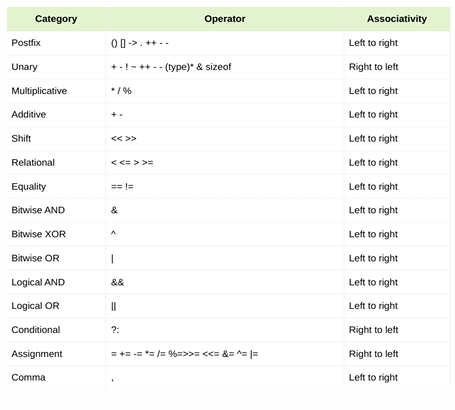
\includegraphics[width=0.65\textwidth]{figuresP/lesson_parallel_3a_pag_21.png}
\end{center}

\subsection{Control Flow and Output}

With operators at our disposal, we can now control the flow of our programs. If you are comfortable with Python, you will find C's control flow highly familiar in its logic, though noticeably different in its syntax. Let's explore conditional statements, loops, and how to properly print our results. As always, you should try and write for yourself the pieces of code at the end of each paragraph.

\subsubsection{- Conditional Statements: if, else, switch}

The fundamental \texttt{if/else} logic is practically identical to Python, but with two major syntax differences: conditions must be enclosed in parentheses \texttt{()}, and blocks of code are defined by braces \texttt{\{\}} instead of indentation. It is always a best practice to "protect" your \texttt{if} statements with braces even if they contain only a single line of code.

Crucially, C does not have an \texttt{elif} keyword. Instead, you simply chain them using \texttt{else if}.

C also provides two other ways to handle conditionals:
\begin{itemize}
    \item \textbf{The Ternary Operator (\texttt{?:}):} A compact, inline \texttt{if/else} statement. The syntax is \texttt{(expression) ? (return if true) : (return if false)}. It is the C equivalent of Python's \texttt{x if condition else y}.
    \item \textbf{The \texttt{switch/case} statement:} When you need to match a single variable against multiple constant values, a \texttt{switch} block is much cleaner than a long chain of \texttt{else if} statements. Remember to use the \texttt{break} keyword at the end of each \texttt{case}, otherwise the execution will "fall through" and execute the subsequent cases as well!
\end{itemize}

\begin{Verbatim}[label=\makebox{\url{https://github.com/lucabaldini/cmepda/tree/master/slides/latex/snippets/control_flow.c}},commandchars=\\\{\}]
\PY{c+cp}{\#}\PY{c+cp}{include}\PY{+w}{ }\PY{c+cpf}{\PYZlt{}stdio.h\PYZgt{}}

\PY{k+kt}{int}\PY{+w}{ }\PY{n+nf}{main}\PY{p}{(}\PY{p}{)}\PY{+w}{ }\PY{p}{\PYZob{}}
\PY{+w}{    }\PY{k+kt}{int}\PY{+w}{ }\PY{n}{a}\PY{+w}{ }\PY{o}{=}\PY{+w}{ }\PY{l+m+mi}{10}\PY{p}{;}
\PY{+w}{    }\PY{k+kt}{int}\PY{+w}{ }\PY{n}{b}\PY{+w}{ }\PY{o}{=}\PY{+w}{ }\PY{l+m+mi}{7}\PY{p}{;}

\PY{+w}{    }\PY{c+c1}{// if / else if / else}
\PY{+w}{    }\PY{k}{if}\PY{+w}{ }\PY{p}{(}\PY{n}{a}\PY{+w}{ }\PY{o}{=}\PY{o}{=}\PY{+w}{ }\PY{n}{b}\PY{p}{)}\PY{+w}{ }\PY{p}{\PYZob{}}
\PY{+w}{        }\PY{n}{printf}\PY{p}{(}\PY{l+s}{\PYZdq{}}\PY{l+s}{a and b are equal}\PY{l+s+se}{\PYZbs{}n}\PY{l+s}{\PYZdq{}}\PY{p}{)}\PY{p}{;}
\PY{+w}{    }\PY{p}{\PYZcb{}}\PY{+w}{ }\PY{k}{else}\PY{+w}{ }\PY{k}{if}\PY{+w}{ }\PY{p}{(}\PY{n}{a}\PY{+w}{ }\PY{o}{\PYZgt{}}\PY{+w}{ }\PY{n}{b}\PY{p}{)}\PY{+w}{ }\PY{p}{\PYZob{}}
\PY{+w}{        }\PY{n}{printf}\PY{p}{(}\PY{l+s}{\PYZdq{}}\PY{l+s}{a is greater}\PY{l+s+se}{\PYZbs{}n}\PY{l+s}{\PYZdq{}}\PY{p}{)}\PY{p}{;}
\PY{+w}{    }\PY{p}{\PYZcb{}}\PY{+w}{ }\PY{k}{else}\PY{+w}{ }\PY{p}{\PYZob{}}
\PY{+w}{        }\PY{n}{printf}\PY{p}{(}\PY{l+s}{\PYZdq{}}\PY{l+s}{b is greater}\PY{l+s+se}{\PYZbs{}n}\PY{l+s}{\PYZdq{}}\PY{p}{)}\PY{p}{;}
\PY{+w}{    }\PY{p}{\PYZcb{}}

\PY{+w}{    }\PY{c+c1}{// Ternary operator ?:}
\PY{+w}{    }\PY{n}{printf}\PY{p}{(}\PY{l+s}{\PYZdq{}}\PY{l+s}{a and b are }\PY{l+s}{\PYZdq{}}\PY{p}{)}\PY{p}{;}
\PY{+w}{    }\PY{n}{printf}\PY{p}{(}\PY{p}{(}\PY{n}{a}\PY{+w}{ }\PY{o}{=}\PY{o}{=}\PY{+w}{ }\PY{n}{b}\PY{p}{)}\PY{+w}{ }\PY{o}{?}\PY{+w}{ }\PY{l+s}{\PYZdq{}}\PY{l+s}{equal}\PY{l+s+se}{\PYZbs{}n}\PY{l+s}{\PYZdq{}}\PY{+w}{ }\PY{o}{:}\PY{+w}{ }\PY{l+s}{\PYZdq{}}\PY{l+s}{different}\PY{l+s+se}{\PYZbs{}n}\PY{l+s}{\PYZdq{}}\PY{p}{)}\PY{p}{;}

\PY{+w}{    }\PY{c+c1}{// Switch/case}
\PY{+w}{    }\PY{k+kt}{int}\PY{+w}{ }\PY{n}{choice}\PY{+w}{ }\PY{o}{=}\PY{+w}{ }\PY{l+m+mi}{2}\PY{p}{;}
\PY{+w}{    }\PY{k}{switch}\PY{+w}{ }\PY{p}{(}\PY{n}{choice}\PY{p}{)}\PY{+w}{ }\PY{p}{\PYZob{}}
\PY{+w}{        }\PY{k}{case}\PY{+w}{ }\PY{l+m+mi}{1}\PY{p}{:}
\PY{+w}{            }\PY{n}{printf}\PY{p}{(}\PY{l+s}{\PYZdq{}}\PY{l+s}{You chose 1}\PY{l+s+se}{\PYZbs{}n}\PY{l+s}{\PYZdq{}}\PY{p}{)}\PY{p}{;}
\PY{+w}{            }\PY{k}{break}\PY{p}{;}
\PY{+w}{        }\PY{k}{case}\PY{+w}{ }\PY{l+m+mi}{2}\PY{p}{:}
\PY{+w}{            }\PY{n}{printf}\PY{p}{(}\PY{l+s}{\PYZdq{}}\PY{l+s}{You chose 2}\PY{l+s+se}{\PYZbs{}n}\PY{l+s}{\PYZdq{}}\PY{p}{)}\PY{p}{;}
\PY{+w}{            }\PY{k}{break}\PY{p}{;}\PY{+w}{ }\PY{c+c1}{// Try removing this break to see the \PYZdq{}fall through\PYZdq{} effect!}
\PY{+w}{        }\PY{k}{default}\PY{o}{:}
\PY{+w}{            }\PY{n}{printf}\PY{p}{(}\PY{l+s}{\PYZdq{}}\PY{l+s}{Invalid choice}\PY{l+s+se}{\PYZbs{}n}\PY{l+s}{\PYZdq{}}\PY{p}{)}\PY{p}{;}
\PY{+w}{    }\PY{p}{\PYZcb{}}

\PY{+w}{    }\PY{k}{return}\PY{+w}{ }\PY{l+m+mi}{0}\PY{p}{;}
\PY{p}{\PYZcb{}}

[Output]
a is greater
a and b are different
You chose 2
\end{Verbatim}

\subsubsection{- The \texttt{printf} Function}

So far, we have used \texttt{printf} without properly introducing it. While Python's \texttt{print()} or f-strings automatically handle different data types, C requires you to explicitly declare the type of the variables you want to print using a \textbf{format string}.

Placeholders inside the string start with \texttt{\%} and are followed by a specific letter depending on the variable's type. The variables are then passed as subsequent arguments. Some of the most common specifiers include:
\begin{itemize}
    \item \texttt{\%d} or \texttt{\%i}: Decimal integer
    \item \texttt{\%f}: Floating point number
    \item \texttt{\%c}: Single character
    \item \texttt{\%s}: String of characters
\end{itemize}

Just like in Python, you can specify complex formatting, such as the number of decimal digits or leading zeroes (e.g., \texttt{\%.2f} for a float with two decimal places).

\begin{Verbatim}[label=\makebox{\url{https://github.com/lucabaldini/cmepda/tree/master/slides/latex/snippets/printf_formatting.c}},commandchars=\\\{\}]
\PY{c+cp}{\#}\PY{c+cp}{include}\PY{+w}{ }\PY{c+cpf}{\PYZlt{}stdio.h\PYZgt{}}

\PY{k+kt}{int}\PY{+w}{ }\PY{n+nf}{main}\PY{p}{(}\PY{p}{)}\PY{+w}{ }\PY{p}{\PYZob{}}
\PY{+w}{    }\PY{k+kt}{int}\PY{+w}{ }\PY{n}{age}\PY{+w}{ }\PY{o}{=}\PY{+w}{ }\PY{l+m+mi}{25}\PY{p}{;}
\PY{+w}{    }\PY{k+kt}{float}\PY{+w}{ }\PY{n}{pi}\PY{+w}{ }\PY{o}{=}\PY{+w}{ }\PY{l+m+mf}{3.14159f}\PY{p}{;}
\PY{+w}{    }\PY{k+kt}{char}\PY{+w}{ }\PY{n}{grade}\PY{+w}{ }\PY{o}{=}\PY{+w}{ }\PY{l+s+sc}{\PYZsq{}}\PY{l+s+sc}{A}\PY{l+s+sc}{\PYZsq{}}\PY{p}{;}

\PY{+w}{    }\PY{c+c1}{// Basic formatting}
\PY{+w}{    }\PY{n}{printf}\PY{p}{(}\PY{l+s}{\PYZdq{}}\PY{l+s}{I am \PYZpc{}d years old.}\PY{l+s+se}{\PYZbs{}n}\PY{l+s}{\PYZdq{}}\PY{p}{,}\PY{+w}{ }\PY{n}{age}\PY{p}{)}\PY{p}{;}
\PY{+w}{    }\PY{n}{printf}\PY{p}{(}\PY{l+s}{\PYZdq{}}\PY{l+s}{The value of pi is \PYZpc{}f.}\PY{l+s+se}{\PYZbs{}n}\PY{l+s}{\PYZdq{}}\PY{p}{,}\PY{+w}{ }\PY{n}{pi}\PY{p}{)}\PY{p}{;}
\PY{+w}{    }\PY{n}{printf}\PY{p}{(}\PY{l+s}{\PYZdq{}}\PY{l+s}{My grade is \PYZpc{}c.}\PY{l+s+se}{\PYZbs{}n}\PY{l+s}{\PYZdq{}}\PY{p}{,}\PY{+w}{ }\PY{n}{grade}\PY{p}{)}\PY{p}{;}

\PY{+w}{    }\PY{c+c1}{// Advanced formatting (precision and padding)}
\PY{+w}{    }\PY{n}{printf}\PY{p}{(}\PY{l+s}{\PYZdq{}}\PY{l+s}{Pi rounded to 2 decimals: \PYZpc{}.2f}\PY{l+s+se}{\PYZbs{}n}\PY{l+s}{\PYZdq{}}\PY{p}{,}\PY{+w}{ }\PY{n}{pi}\PY{p}{)}\PY{p}{;}
\PY{+w}{    }\PY{n}{printf}\PY{p}{(}\PY{l+s}{\PYZdq{}}\PY{l+s}{Padded integer: \PYZpc{}05d}\PY{l+s+se}{\PYZbs{}n}\PY{l+s}{\PYZdq{}}\PY{p}{,}\PY{+w}{ }\PY{n}{age}\PY{p}{)}\PY{p}{;}\PY{+w}{ }\PY{c+c1}{// Prints 00025}

\PY{+w}{    }\PY{c+c1}{// Multiple variables}
\PY{+w}{    }\PY{n}{printf}\PY{p}{(}\PY{l+s}{\PYZdq{}}\PY{l+s}{Values: \PYZpc{}d, \PYZpc{}.1f, \PYZpc{}c}\PY{l+s+se}{\PYZbs{}n}\PY{l+s}{\PYZdq{}}\PY{p}{,}\PY{+w}{ }\PY{n}{age}\PY{p}{,}\PY{+w}{ }\PY{n}{pi}\PY{p}{,}\PY{+w}{ }\PY{n}{grade}\PY{p}{)}\PY{p}{;}

\PY{+w}{    }\PY{k}{return}\PY{+w}{ }\PY{l+m+mi}{0}\PY{p}{;}
\PY{p}{\PYZcb{}}

[Output]
I am 25 years old.
The value of pi is 3.141590.
My grade is A.
Pi rounded to 2 decimals: 3.14
Padded integer: 00025
Values: 25, 3.1, A
\end{Verbatim}

\subsubsection{- Loops: for, while, do...while}

This is where Python programmers usually face a small learning curve. Python's \texttt{for} loop is actually a "for-each" loop, designed to iterate over collections (like lists or ranges). C's \texttt{for} loop, instead, is explicitly mechanical and controlled by three statements separated by semicolons: \texttt{for(initialization; condition; repeated action)}.
\begin{itemize}
    \item \textbf{Initialization:} Executed only once before the loop starts (e.g., \texttt{int i = 0}).
    \item \textbf{Condition:} Evaluated before every iteration. If true, the loop runs (e.g., \texttt{i < 10}).
    \item \textbf{Repeated action:} Executed at the end of every iteration (e.g., \texttt{i++}).
\end{itemize}

The \texttt{while} loop behaves exactly as it does in Python: it checks the condition \textit{before} the iteration starts.

C also introduces the \textbf{\texttt{do...while}} loop. The critical difference here is that the condition is checked \textit{after} the iteration. This guarantees that the code block inside a \texttt{do...while} loop is executed \textbf{at least once}, even if the condition is completely false from the very beginning.

Finally, the \texttt{break} (to exit the loop entirely) and \texttt{continue} (to skip the rest of the current iteration and proceed to the next) keywords work exactly as they do in Python.

\begin{Verbatim}[label=\makebox{\url{https://github.com/lucabaldini/cmepda/tree/master/slides/latex/snippets/loops.c}},commandchars=\\\{\}]
\PY{c+cp}{\#}\PY{c+cp}{include}\PY{+w}{ }\PY{c+cpf}{\PYZlt{}stdio.h\PYZgt{}}

\PY{k+kt}{int}\PY{+w}{ }\PY{n+nf}{main}\PY{p}{(}\PY{p}{)}\PY{+w}{ }\PY{p}{\PYZob{}}
\PY{+w}{    }\PY{c+c1}{// 1. FOR LOOP}
\PY{+w}{    }\PY{n}{printf}\PY{p}{(}\PY{l+s}{\PYZdq{}}\PY{l+s}{\PYZhy{}\PYZhy{}\PYZhy{} For Loop \PYZhy{}\PYZhy{}\PYZhy{}}\PY{l+s+se}{\PYZbs{}n}\PY{l+s}{\PYZdq{}}\PY{p}{)}\PY{p}{;}
\PY{+w}{    }\PY{k}{for}\PY{+w}{ }\PY{p}{(}\PY{k+kt}{int}\PY{+w}{ }\PY{n}{i}\PY{+w}{ }\PY{o}{=}\PY{+w}{ }\PY{l+m+mi}{0}\PY{p}{;}\PY{+w}{ }\PY{n}{i}\PY{+w}{ }\PY{o}{\PYZlt{}}\PY{+w}{ }\PY{l+m+mi}{3}\PY{p}{;}\PY{+w}{ }\PY{n}{i}\PY{o}{+}\PY{o}{+}\PY{p}{)}\PY{+w}{ }\PY{p}{\PYZob{}}
\PY{+w}{        }\PY{n}{printf}\PY{p}{(}\PY{l+s}{\PYZdq{}}\PY{l+s}{Iteration \PYZpc{}d}\PY{l+s+se}{\PYZbs{}n}\PY{l+s}{\PYZdq{}}\PY{p}{,}\PY{+w}{ }\PY{n}{i}\PY{p}{)}\PY{p}{;}
\PY{+w}{    }\PY{p}{\PYZcb{}}
\PY{+w}{    }
\PY{+w}{    }\PY{c+c1}{// 2. BREAK AND CONTINUE}
\PY{+w}{    }\PY{n}{printf}\PY{p}{(}\PY{l+s}{\PYZdq{}}\PY{l+s+se}{\PYZbs{}n}\PY{l+s}{\PYZhy{}\PYZhy{}\PYZhy{} Break \PYZam{} Continue \PYZhy{}\PYZhy{}\PYZhy{}}\PY{l+s+se}{\PYZbs{}n}\PY{l+s}{\PYZdq{}}\PY{p}{)}\PY{p}{;}
\PY{+w}{    }\PY{k}{for}\PY{+w}{ }\PY{p}{(}\PY{k+kt}{int}\PY{+w}{ }\PY{n}{i}\PY{+w}{ }\PY{o}{=}\PY{+w}{ }\PY{l+m+mi}{0}\PY{p}{;}\PY{+w}{ }\PY{n}{i}\PY{+w}{ }\PY{o}{\PYZlt{}}\PY{+w}{ }\PY{l+m+mi}{10}\PY{p}{;}\PY{+w}{ }\PY{n}{i}\PY{o}{+}\PY{o}{+}\PY{p}{)}\PY{+w}{ }\PY{p}{\PYZob{}}
\PY{+w}{        }\PY{k}{if}\PY{+w}{ }\PY{p}{(}\PY{n}{i}\PY{+w}{ }\PY{o}{\PYZgt{}}\PY{+w}{ }\PY{l+m+mi}{5}\PY{p}{)}\PY{+w}{ }\PY{k}{break}\PY{p}{;}\PY{+w}{       }\PY{c+c1}{// Exit loop if i \PYZgt{} 5}
\PY{+w}{        }\PY{k}{if}\PY{+w}{ }\PY{p}{(}\PY{n}{i}\PY{+w}{ }\PY{o}{\PYZgt{}}\PY{+w}{ }\PY{l+m+mi}{2}\PY{p}{)}\PY{+w}{ }\PY{k}{continue}\PY{p}{;}\PY{+w}{    }\PY{c+c1}{// Skip print if i \PYZgt{} 2 (but i \PYZlt{}= 5)}
\PY{+w}{        }\PY{n}{printf}\PY{p}{(}\PY{l+s}{\PYZdq{}}\PY{l+s}{Hi there, i is \PYZpc{}d}\PY{l+s+se}{\PYZbs{}n}\PY{l+s}{\PYZdq{}}\PY{p}{,}\PY{+w}{ }\PY{n}{i}\PY{p}{)}\PY{p}{;}\PY{+w}{ }
\PY{+w}{    }\PY{p}{\PYZcb{}}
\PY{+w}{    }
\PY{+w}{    }\PY{c+c1}{// 3. WHILE vs DO...WHILE}
\PY{+w}{    }\PY{n}{printf}\PY{p}{(}\PY{l+s}{\PYZdq{}}\PY{l+s+se}{\PYZbs{}n}\PY{l+s}{\PYZhy{}\PYZhy{}\PYZhy{} While vs Do...While \PYZhy{}\PYZhy{}\PYZhy{}}\PY{l+s+se}{\PYZbs{}n}\PY{l+s}{\PYZdq{}}\PY{p}{)}\PY{p}{;}
\PY{+w}{    }
\PY{+w}{    }\PY{k+kt}{int}\PY{+w}{ }\PY{n}{j}\PY{+w}{ }\PY{o}{=}\PY{+w}{ }\PY{l+m+mi}{0}\PY{p}{;}
\PY{+w}{    }\PY{k}{while}\PY{+w}{ }\PY{p}{(}\PY{n}{j}\PY{+w}{ }\PY{o}{\PYZlt{}}\PY{+w}{ }\PY{l+m+mi}{0}\PY{p}{)}\PY{+w}{ }\PY{p}{\PYZob{}}\PY{+w}{  }\PY{c+c1}{// Condition is false to start with!}
\PY{+w}{        }\PY{n}{j}\PY{o}{+}\PY{o}{+}\PY{p}{;}
\PY{+w}{        }\PY{n}{printf}\PY{p}{(}\PY{l+s}{\PYZdq{}}\PY{l+s}{while: j=\PYZpc{}d}\PY{l+s+se}{\PYZbs{}n}\PY{l+s}{\PYZdq{}}\PY{p}{,}\PY{+w}{ }\PY{n}{j}\PY{p}{)}\PY{p}{;}\PY{+w}{ }\PY{c+c1}{// This will never print}
\PY{+w}{    }\PY{p}{\PYZcb{}}
\PY{+w}{    }
\PY{+w}{    }\PY{k+kt}{int}\PY{+w}{ }\PY{n}{k}\PY{+w}{ }\PY{o}{=}\PY{+w}{ }\PY{l+m+mi}{0}\PY{p}{;}
\PY{+w}{    }\PY{k}{do}\PY{+w}{ }\PY{p}{\PYZob{}}\PY{+w}{             }\PY{c+c1}{// Condition is false, but executes once!}
\PY{+w}{        }\PY{n}{k}\PY{o}{+}\PY{o}{+}\PY{p}{;}
\PY{+w}{        }\PY{n}{printf}\PY{p}{(}\PY{l+s}{\PYZdq{}}\PY{l+s}{do...while: k=\PYZpc{}d}\PY{l+s+se}{\PYZbs{}n}\PY{l+s}{\PYZdq{}}\PY{p}{,}\PY{+w}{ }\PY{n}{k}\PY{p}{)}\PY{p}{;}\PY{+w}{ }
\PY{+w}{    }\PY{p}{\PYZcb{}}\PY{+w}{ }\PY{k}{while}\PY{+w}{ }\PY{p}{(}\PY{n}{k}\PY{+w}{ }\PY{o}{\PYZlt{}}\PY{+w}{ }\PY{l+m+mi}{0}\PY{p}{)}\PY{p}{;}
\PY{+w}{    }
\PY{+w}{    }\PY{n}{printf}\PY{p}{(}\PY{l+s}{\PYZdq{}}\PY{l+s}{After loops, j is \PYZpc{}d and k is \PYZpc{}d}\PY{l+s+se}{\PYZbs{}n}\PY{l+s}{\PYZdq{}}\PY{p}{,}\PY{+w}{ }\PY{n}{j}\PY{p}{,}\PY{+w}{ }\PY{n}{k}\PY{p}{)}\PY{p}{;}
\PY{+w}{    }
\PY{+w}{    }\PY{k}{return}\PY{+w}{ }\PY{l+m+mi}{0}\PY{p}{;}
\PY{p}{\PYZcb{}}

[Output]
--- For Loop ---
Iteration 0
Iteration 1
Iteration 2

--- Break & Continue ---
Hi there, i is 0
Hi there, i is 1
Hi there, i is 2

--- While vs Do...While ---
do...while: k=1
After loops, j is 0 and k is 1
\end{Verbatim}

\subsection{Functions and Scope}

In Python, defining a function is as simple as using the \texttt{def} keyword. In C, functions require a bit more structure. A C function consists of a \textbf{signature} (its name, the number of parameters, and their types) and a \textbf{body} (the actual code block). Furthermore, every function must specify a \textbf{return type}; if the function does not return anything, the type must be declared as \texttt{void}.

A crucial difference from Python is the distinction between \textbf{defining} and \textbf{declaring} a function:
\begin{itemize}
    \item \textbf{Defining:} Writing the full function, including its body.
    \item \textbf{Declaring:} Providing only the signature to the compiler, usually at the top of the file or in a header file.
\end{itemize}
Why declare? The C compiler reads code from top to bottom. If function A calls function B, function B must be known to the compiler beforehand. Declaring allows you to inform the compiler that a function exists and what it looks like, even if its actual definition is written further down in the file (or in a completely different file). This is essential for mutually recursive functions.

Another major difference is \textbf{variable scope}. While Python's scope is mostly tied to functions and modules, C uses \textbf{block scope}: variables strictly exist only within the block \texttt{\{\}} where they are declared. If you declare a variable inside a nested block with the same name as one outside of it, the inner variable will "hide" the outer one until the block ends. Here's an example:

\begin{Verbatim}[label=\makebox{\url{https://github.com/lucabaldini/cmepda/tree/master/slides/latex/snippets/functions_and_scope.c}},commandchars=\\\{\}]
\PY{c+cp}{\#}\PY{c+cp}{include}\PY{+w}{ }\PY{c+cpf}{\PYZlt{}stdio.h\PYZgt{}}
\PY{c+cp}{\#}\PY{c+cp}{include}\PY{+w}{ }\PY{c+cpf}{\PYZlt{}stdbool.h\PYZgt{}}

\PY{c+c1}{// 1. Declaration (providing the signature before definition)}
\PY{k+kt}{bool}\PY{+w}{ }\PY{n}{isEven}\PY{p}{(}\PY{k+kt}{int}\PY{+w}{ }\PY{n}{n}\PY{p}{)}\PY{p}{;}

\PY{c+c1}{// 2. Definition}
\PY{k+kt}{bool}\PY{+w}{ }\PY{n+nf}{isOdd}\PY{p}{(}\PY{k+kt}{int}\PY{+w}{ }\PY{n}{n}\PY{p}{)}\PY{+w}{ }\PY{p}{\PYZob{}}
\PY{+w}{    }\PY{k}{if}\PY{+w}{ }\PY{p}{(}\PY{n}{n}\PY{+w}{ }\PY{o}{=}\PY{o}{=}\PY{+w}{ }\PY{l+m+mi}{0}\PY{p}{)}\PY{+w}{ }\PY{k}{return}\PY{+w}{ }\PY{n+nb}{false}\PY{p}{;}
\PY{+w}{    }\PY{c+c1}{// Calls isEven, which the compiler knows about thanks to the declaration}
\PY{+w}{    }\PY{k}{return}\PY{+w}{ }\PY{n}{isEven}\PY{p}{(}\PY{n}{n}\PY{+w}{ }\PY{o}{\PYZhy{}}\PY{+w}{ }\PY{l+m+mi}{1}\PY{p}{)}\PY{p}{;}
\PY{p}{\PYZcb{}}

\PY{k+kt}{bool}\PY{+w}{ }\PY{n+nf}{isEven}\PY{p}{(}\PY{k+kt}{int}\PY{+w}{ }\PY{n}{n}\PY{p}{)}\PY{+w}{ }\PY{p}{\PYZob{}}
\PY{+w}{    }\PY{k}{if}\PY{+w}{ }\PY{p}{(}\PY{n}{n}\PY{+w}{ }\PY{o}{=}\PY{o}{=}\PY{+w}{ }\PY{l+m+mi}{0}\PY{p}{)}\PY{+w}{ }\PY{k}{return}\PY{+w}{ }\PY{n+nb}{true}\PY{p}{;}
\PY{+w}{    }\PY{k}{return}\PY{+w}{ }\PY{n}{isOdd}\PY{p}{(}\PY{n}{n}\PY{+w}{ }\PY{o}{\PYZhy{}}\PY{+w}{ }\PY{l+m+mi}{1}\PY{p}{)}\PY{p}{;}
\PY{p}{\PYZcb{}}

\PY{k+kt}{int}\PY{+w}{ }\PY{n+nf}{main}\PY{p}{(}\PY{p}{)}\PY{+w}{ }\PY{p}{\PYZob{}}
\PY{+w}{    }\PY{k+kt}{int}\PY{+w}{ }\PY{n}{a}\PY{+w}{ }\PY{o}{=}\PY{+w}{ }\PY{l+m+mi}{1}\PY{p}{;}
\PY{+w}{    }\PY{k+kt}{int}\PY{+w}{ }\PY{n}{b}\PY{+w}{ }\PY{o}{=}\PY{+w}{ }\PY{l+m+mi}{10}\PY{p}{;}
\PY{+w}{    }
\PY{+w}{    }\PY{c+c1}{// 3. Variable Scope}
\PY{+w}{    }\PY{p}{\PYZob{}}\PY{+w}{ }\PY{c+c1}{// Start of a new nested block}
\PY{+w}{        }\PY{k+kt}{int}\PY{+w}{ }\PY{n}{a}\PY{+w}{ }\PY{o}{=}\PY{+w}{ }\PY{l+m+mi}{100}\PY{p}{;}\PY{+w}{ }\PY{c+c1}{// This \PYZsq{}a\PYZsq{} hides the outer \PYZsq{}a\PYZsq{}}
\PY{+w}{        }\PY{k+kt}{int}\PY{+w}{ }\PY{n}{c}\PY{+w}{ }\PY{o}{=}\PY{+w}{ }\PY{l+m+mi}{10000}\PY{p}{;}
\PY{+w}{        }\PY{n}{printf}\PY{p}{(}\PY{l+s}{\PYZdq{}}\PY{l+s}{Inner block: a = \PYZpc{}d, b = \PYZpc{}d}\PY{l+s+se}{\PYZbs{}n}\PY{l+s}{\PYZdq{}}\PY{p}{,}\PY{+w}{ }\PY{n}{a}\PY{p}{,}\PY{+w}{ }\PY{n}{b}\PY{p}{)}\PY{p}{;}
\PY{+w}{    }\PY{p}{\PYZcb{}}\PY{+w}{ }\PY{c+c1}{// \PYZsq{}c\PYZsq{} is destroyed here, and the inner \PYZsq{}a\PYZsq{} is destroyed}
\PY{+w}{    }
\PY{+w}{    }\PY{n}{printf}\PY{p}{(}\PY{l+s}{\PYZdq{}}\PY{l+s}{Outer block: a = \PYZpc{}d}\PY{l+s+se}{\PYZbs{}n}\PY{l+s}{\PYZdq{}}\PY{p}{,}\PY{+w}{ }\PY{n}{a}\PY{p}{)}\PY{p}{;}
\PY{+w}{    }\PY{c+c1}{// printf(\PYZdq{}\PYZpc{}d\PYZdq{}, c); // This would cause a compile error: \PYZsq{}c\PYZsq{} undeclared}
\PY{+w}{    }
\PY{+w}{    }\PY{n}{printf}\PY{p}{(}\PY{l+s}{\PYZdq{}}\PY{l+s}{Is 17 even? \PYZpc{}s}\PY{l+s+se}{\PYZbs{}n}\PY{l+s}{\PYZdq{}}\PY{p}{,}\PY{+w}{ }\PY{n}{isEven}\PY{p}{(}\PY{l+m+mi}{17}\PY{p}{)}\PY{+w}{ }\PY{o}{?}\PY{+w}{ }\PY{l+s}{\PYZdq{}}\PY{l+s}{true}\PY{l+s}{\PYZdq{}}\PY{+w}{ }\PY{o}{:}\PY{+w}{ }\PY{l+s}{\PYZdq{}}\PY{l+s}{false}\PY{l+s}{\PYZdq{}}\PY{p}{)}\PY{p}{;}
\PY{+w}{    }
\PY{+w}{    }\PY{k}{return}\PY{+w}{ }\PY{l+m+mi}{0}\PY{p}{;}
\PY{p}{\PYZcb{}}

[Output]
Inner block: a = 100, b = 10
Outer block: a = 1
Is 17 even? false
\end{Verbatim}

\subsection{Variables, Memory, and Pointers}

To truly understand C, you must understand how it manages memory. Unlike Python, which hides memory management through automatic garbage collection, C forces you to be aware of where your data lives. Variables are stored in RAM using two primary mechanisms:
\begin{itemize}
    \item \textbf{Stack:} Operates in a LIFO (Last In, First Out) order. It is fast, automatic, and used for local variables and function arguments. When a function finishes, its stack memory is immediately freed.
    \item \textbf{Heap:} Memory allocated explicitly by the user (using functions like \texttt{malloc}). This memory survives until you explicitly release it (using \texttt{free}), making it essential for data that must outlive the function that created it.
\end{itemize}

Every variable is stored at a precise location in memory, called its \textbf{address}. A \textbf{pointer} is simply a special type of variable that stores a memory address instead of a standard value.
\begin{itemize}
    \item The \textbf{\texttt{\&}} operator returns the memory address of a variable.
    \item The \textbf{\texttt{*}} operator, when used in declaration (e.g., \texttt{int *p}), denotes a pointer type. When used in front of an existing pointer, it "dereferences" it, allowing you to access or modify the value stored at that memory address.
\end{itemize}

Pointers are the only way to modify variables passed to a function. C functions strictly pass arguments \textbf{by value} (they create local copies). If you want a function to modify an original variable, you must pass its memory address (a pointer) so the function knows exactly where to look.

\begin{Verbatim}[label=\makebox{\url{https://github.com/lucabaldini/cmepda/tree/master/slides/latex/snippets/pointers.c}},commandchars=\\\{\}]
\PY{c+cp}{\#}\PY{c+cp}{include}\PY{+w}{ }\PY{c+cpf}{\PYZlt{}stdio.h\PYZgt{}}

\PY{c+c1}{// Pass by value (creates a local copy, cannot modify original)}
\PY{k+kt}{int}\PY{+w}{ }\PY{n+nf}{notIncrement}\PY{p}{(}\PY{k+kt}{int}\PY{+w}{ }\PY{n}{i}\PY{p}{)}\PY{+w}{ }\PY{p}{\PYZob{}}
\PY{+w}{    }\PY{n}{i}\PY{+w}{ }\PY{o}{+}\PY{o}{=}\PY{+w}{ }\PY{l+m+mi}{1}\PY{p}{;}
\PY{+w}{    }\PY{k}{return}\PY{+w}{ }\PY{n}{i}\PY{p}{;}
\PY{p}{\PYZcb{}}

\PY{c+c1}{// Pass by pointer (receives the address, modifies original data)}
\PY{k+kt}{int}\PY{+w}{ }\PY{n+nf}{increment}\PY{p}{(}\PY{k+kt}{int}\PY{+w}{ }\PY{o}{*}\PY{n}{i}\PY{p}{)}\PY{+w}{ }\PY{p}{\PYZob{}}
\PY{+w}{    }\PY{p}{(}\PY{o}{*}\PY{n}{i}\PY{p}{)}\PY{+w}{ }\PY{o}{+}\PY{o}{=}\PY{+w}{ }\PY{l+m+mi}{1}\PY{p}{;}\PY{+w}{ }\PY{c+c1}{// Dereference the pointer to modify the actual value}
\PY{+w}{    }\PY{k}{return}\PY{+w}{ }\PY{o}{*}\PY{n}{i}\PY{p}{;}
\PY{p}{\PYZcb{}}

\PY{k+kt}{int}\PY{+w}{ }\PY{n+nf}{main}\PY{p}{(}\PY{p}{)}\PY{+w}{ }\PY{p}{\PYZob{}}
\PY{+w}{    }\PY{k+kt}{float}\PY{+w}{ }\PY{n}{a}\PY{+w}{ }\PY{o}{=}\PY{+w}{ }\PY{l+m+mf}{0.0f}\PY{p}{;}
\PY{+w}{    }\PY{k+kt}{float}\PY{+w}{ }\PY{n}{b}\PY{+w}{ }\PY{o}{=}\PY{+w}{ }\PY{l+m+mf}{0.0f}\PY{p}{;}
\PY{+w}{    }\PY{k+kt}{float}\PY{+w}{ }\PY{o}{*}\PY{n}{ap}\PY{+w}{ }\PY{o}{=}\PY{+w}{ }\PY{o}{\PYZam{}}\PY{n}{a}\PY{p}{;}\PY{+w}{ }\PY{c+c1}{// \PYZsq{}ap\PYZsq{} holds the memory address of \PYZsq{}a\PYZsq{}}
\PY{+w}{    }
\PY{+w}{    }\PY{n}{printf}\PY{p}{(}\PY{l+s}{\PYZdq{}}\PY{l+s}{a: \PYZpc{}f, ap points to: \PYZpc{}f}\PY{l+s+se}{\PYZbs{}n}\PY{l+s}{\PYZdq{}}\PY{p}{,}\PY{+w}{ }\PY{n}{a}\PY{p}{,}\PY{+w}{ }\PY{o}{*}\PY{n}{ap}\PY{p}{)}\PY{p}{;}
\PY{+w}{    }
\PY{+w}{    }\PY{n}{a}\PY{+w}{ }\PY{o}{=}\PY{+w}{ }\PY{l+m+mf}{1.0f}\PY{p}{;}
\PY{+w}{    }\PY{n}{printf}\PY{p}{(}\PY{l+s}{\PYZdq{}}\PY{l+s}{a: \PYZpc{}f, ap points to: \PYZpc{}f}\PY{l+s+se}{\PYZbs{}n}\PY{l+s}{\PYZdq{}}\PY{p}{,}\PY{+w}{ }\PY{n}{a}\PY{p}{,}\PY{+w}{ }\PY{o}{*}\PY{n}{ap}\PY{p}{)}\PY{p}{;}\PY{+w}{ }\PY{c+c1}{// Changing \PYZsq{}a\PYZsq{} changes \PYZsq{}*ap\PYZsq{}}
\PY{+w}{    }
\PY{+w}{    }\PY{o}{*}\PY{n}{ap}\PY{+w}{ }\PY{o}{=}\PY{+w}{ }\PY{l+m+mf}{2.0f}\PY{p}{;}\PY{+w}{ }\PY{c+c1}{// Modifying the value stored at the address pointed by \PYZsq{}ap\PYZsq{}}
\PY{+w}{    }\PY{n}{printf}\PY{p}{(}\PY{l+s}{\PYZdq{}}\PY{l+s}{a: \PYZpc{}f, ap points to: \PYZpc{}f}\PY{l+s+se}{\PYZbs{}n}\PY{l+s}{\PYZdq{}}\PY{p}{,}\PY{+w}{ }\PY{n}{a}\PY{p}{,}\PY{+w}{ }\PY{o}{*}\PY{n}{ap}\PY{p}{)}\PY{p}{;}\PY{+w}{ }\PY{c+c1}{// \PYZsq{}a\PYZsq{} is now 2.0}
\PY{+w}{    }
\PY{+w}{    }\PY{c+c1}{// Passing pointers to functions}
\PY{+w}{    }\PY{k+kt}{int}\PY{+w}{ }\PY{n}{myNum}\PY{+w}{ }\PY{o}{=}\PY{+w}{ }\PY{l+m+mi}{10}\PY{p}{;}
\PY{+w}{    }\PY{n}{printf}\PY{p}{(}\PY{l+s}{\PYZdq{}}\PY{l+s+se}{\PYZbs{}n}\PY{l+s}{Original myNum: \PYZpc{}d}\PY{l+s+se}{\PYZbs{}n}\PY{l+s}{\PYZdq{}}\PY{p}{,}\PY{+w}{ }\PY{n}{myNum}\PY{p}{)}\PY{p}{;}
\PY{+w}{    }\PY{n}{printf}\PY{p}{(}\PY{l+s}{\PYZdq{}}\PY{l+s}{notIncrement returns: \PYZpc{}d | myNum is still: \PYZpc{}d}\PY{l+s+se}{\PYZbs{}n}\PY{l+s}{\PYZdq{}}\PY{p}{,}\PY{+w}{ }\PY{n}{notIncrement}\PY{p}{(}\PY{n}{myNum}\PY{p}{)}\PY{p}{,}\PY{+w}{ }\PY{n}{myNum}\PY{p}{)}\PY{p}{;}
\PY{+w}{    }\PY{n}{printf}\PY{p}{(}\PY{l+s}{\PYZdq{}}\PY{l+s}{increment returns: \PYZpc{}d | myNum is now: \PYZpc{}d}\PY{l+s+se}{\PYZbs{}n}\PY{l+s}{\PYZdq{}}\PY{p}{,}\PY{+w}{ }\PY{n}{increment}\PY{p}{(}\PY{o}{\PYZam{}}\PY{n}{myNum}\PY{p}{)}\PY{p}{,}\PY{+w}{ }\PY{n}{myNum}\PY{p}{)}\PY{p}{;}
\PY{+w}{    }
\PY{+w}{    }\PY{k}{return}\PY{+w}{ }\PY{l+m+mi}{0}\PY{p}{;}
\PY{p}{\PYZcb{}}

[Output]
a: 0.000000, ap points to: 0.000000
a: 1.000000, ap points to: 1.000000
a: 2.000000, ap points to: 2.000000

Original myNum: 10
notIncrement returns: 11 | myNum is still: 10
increment returns: 11 | myNum is now: 11
\end{Verbatim}

\subsection{Arrays and Dynamic Memory}

In C, arrays are not like Python lists: they are fixed-size blocks of contiguous memory. You declare them specifying the type and the size: \texttt{type varName[size];}. 

Arrays and pointers are deeply interconnected. In fact, an array variable often behaves just like a pointer to its first element. You can assign an array to a pointer, and you can access elements using both the \texttt{[]} operator and pointer arithmetic (e.g., \texttt{pointer + N} moves the address forward by N elements).

However, there is a dangerous "gotcha" when combining arrays, pointers, and functions. The \texttt{sizeof} operator usually returns the total memory size of an array. But when you pass an array to a function, it "decays" into a simple pointer. Inside the function, \texttt{sizeof} will only return the size of the pointer itself (usually 8 bytes on modern systems), not the size of the array!

Because C functions can only return a single variable by value, returning an array is tricky. You cannot return an array allocated on the Stack inside a function, because that memory is destroyed the moment the function ends. Instead, you must allocate the array on the Heap using \texttt{malloc} and return a \textbf{pointer} to that surviving memory.

\begin{Verbatim}[label=\makebox{\url{https://github.com/lucabaldini/cmepda/tree/master/slides/latex/snippets/arrays_and_malloc.c}},commandchars=\\\{\}]
\PY{c+cp}{\#}\PY{c+cp}{include}\PY{+w}{ }\PY{c+cpf}{\PYZlt{}stdio.h\PYZgt{}}
\PY{c+cp}{\#}\PY{c+cp}{include}\PY{+w}{ }\PY{c+cpf}{\PYZlt{}stdlib.h\PYZgt{}}\PY{c+c1}{ // Required for malloc and free}

\PY{c+c1}{// Array passed to a function decays to a pointer}
\PY{k+kt}{void}\PY{+w}{ }\PY{n+nf}{printArrayInfo}\PY{p}{(}\PY{k+kt}{int}\PY{+w}{ }\PY{n}{theArray}\PY{p}{[}\PY{p}{]}\PY{p}{)}\PY{+w}{ }\PY{p}{\PYZob{}}
\PY{+w}{    }\PY{c+c1}{// This will print the size of a pointer (usually 8 bytes), NOT the array!}
\PY{+w}{    }\PY{n}{printf}\PY{p}{(}\PY{l+s}{\PYZdq{}}\PY{l+s}{Size inside function: \PYZpc{}lu bytes}\PY{l+s+se}{\PYZbs{}n}\PY{l+s}{\PYZdq{}}\PY{p}{,}\PY{+w}{ }\PY{k}{sizeof}\PY{p}{(}\PY{n}{theArray}\PY{p}{)}\PY{p}{)}\PY{p}{;}\PY{+w}{ }
\PY{p}{\PYZcb{}}

\PY{c+c1}{// Function returning a pointer to dynamically allocated Heap memory}
\PY{k+kt}{char}\PY{+w}{ }\PY{o}{*}\PY{+w}{ }\PY{n+nf}{ones}\PY{p}{(}\PY{k+kt}{int}\PY{+w}{ }\PY{n}{size}\PY{p}{)}\PY{+w}{ }\PY{p}{\PYZob{}}
\PY{+w}{    }\PY{k+kt}{char}\PY{+w}{ }\PY{o}{*}\PY{+w}{ }\PY{n}{ret}\PY{+w}{ }\PY{o}{=}\PY{+w}{ }\PY{n}{malloc}\PY{p}{(}\PY{n}{size}\PY{+w}{ }\PY{o}{*}\PY{+w}{ }\PY{k}{sizeof}\PY{p}{(}\PY{k+kt}{char}\PY{p}{)}\PY{p}{)}\PY{p}{;}\PY{+w}{ }\PY{c+c1}{// Allocate memory explicitly}
\PY{+w}{    }\PY{k}{for}\PY{p}{(}\PY{k+kt}{int}\PY{+w}{ }\PY{n}{i}\PY{+w}{ }\PY{o}{=}\PY{+w}{ }\PY{l+m+mi}{0}\PY{p}{;}\PY{+w}{ }\PY{n}{i}\PY{+w}{ }\PY{o}{\PYZlt{}}\PY{+w}{ }\PY{n}{size}\PY{p}{;}\PY{+w}{ }\PY{n}{i}\PY{o}{+}\PY{o}{+}\PY{p}{)}\PY{+w}{ }\PY{p}{\PYZob{}}
\PY{+w}{        }\PY{n}{ret}\PY{p}{[}\PY{n}{i}\PY{p}{]}\PY{+w}{ }\PY{o}{=}\PY{+w}{ }\PY{l+m+mi}{1}\PY{p}{;}
\PY{+w}{    }\PY{p}{\PYZcb{}}
\PY{+w}{    }\PY{k}{return}\PY{+w}{ }\PY{n}{ret}\PY{p}{;}\PY{+w}{ }\PY{c+c1}{// Returning the pointer is safe because memory is on the Heap}
\PY{p}{\PYZcb{}}

\PY{k+kt}{int}\PY{+w}{ }\PY{n+nf}{main}\PY{p}{(}\PY{p}{)}\PY{+w}{ }\PY{p}{\PYZob{}}
\PY{+w}{    }\PY{c+c1}{// Arrays and Pointers}
\PY{+w}{    }\PY{k+kt}{int}\PY{+w}{ }\PY{n}{anArray}\PY{p}{[}\PY{l+m+mi}{4}\PY{p}{]}\PY{+w}{ }\PY{o}{=}\PY{+w}{ }\PY{p}{\PYZob{}}\PY{l+m+mi}{10}\PY{p}{,}\PY{+w}{ }\PY{l+m+mi}{20}\PY{p}{,}\PY{+w}{ }\PY{l+m+mi}{30}\PY{p}{,}\PY{+w}{ }\PY{l+m+mi}{40}\PY{p}{\PYZcb{}}\PY{p}{;}
\PY{+w}{    }\PY{k+kt}{int}\PY{+w}{ }\PY{o}{*}\PY{n}{p}\PY{+w}{ }\PY{o}{=}\PY{+w}{ }\PY{n}{anArray}\PY{p}{;}\PY{+w}{ }\PY{c+c1}{// Arrays can be directly assigned to pointers}
\PY{+w}{    }
\PY{+w}{    }\PY{n}{printf}\PY{p}{(}\PY{l+s}{\PYZdq{}}\PY{l+s}{Size in main: \PYZpc{}lu bytes}\PY{l+s+se}{\PYZbs{}n}\PY{l+s}{\PYZdq{}}\PY{p}{,}\PY{+w}{ }\PY{k}{sizeof}\PY{p}{(}\PY{n}{anArray}\PY{p}{)}\PY{p}{)}\PY{p}{;}\PY{+w}{ }\PY{c+c1}{// Size of the full array (16 bytes)}
\PY{+w}{    }\PY{n}{printArrayInfo}\PY{p}{(}\PY{n}{anArray}\PY{p}{)}\PY{p}{;}
\PY{+w}{    }
\PY{+w}{    }\PY{c+c1}{// Accessing elements}
\PY{+w}{    }\PY{n}{printf}\PY{p}{(}\PY{l+s}{\PYZdq{}}\PY{l+s+se}{\PYZbs{}n}\PY{l+s}{anArray[2] = \PYZpc{}d}\PY{l+s+se}{\PYZbs{}n}\PY{l+s}{\PYZdq{}}\PY{p}{,}\PY{+w}{ }\PY{n}{anArray}\PY{p}{[}\PY{l+m+mi}{2}\PY{p}{]}\PY{p}{)}\PY{p}{;}
\PY{+w}{    }\PY{n}{printf}\PY{p}{(}\PY{l+s}{\PYZdq{}}\PY{l+s}{p[2] = \PYZpc{}d}\PY{l+s+se}{\PYZbs{}n}\PY{l+s}{\PYZdq{}}\PY{p}{,}\PY{+w}{ }\PY{n}{p}\PY{p}{[}\PY{l+m+mi}{2}\PY{p}{]}\PY{p}{)}\PY{p}{;}\PY{+w}{            }\PY{c+c1}{// [] operator works on pointers}
\PY{+w}{    }\PY{n}{printf}\PY{p}{(}\PY{l+s}{\PYZdq{}}\PY{l+s}{*(p+2) = \PYZpc{}d}\PY{l+s+se}{\PYZbs{}n}\PY{l+s}{\PYZdq{}}\PY{p}{,}\PY{+w}{ }\PY{o}{*}\PY{p}{(}\PY{n}{p}\PY{+w}{ }\PY{o}{+}\PY{+w}{ }\PY{l+m+mi}{2}\PY{p}{)}\PY{p}{)}\PY{p}{;}\PY{+w}{      }\PY{c+c1}{// Pointer arithmetic achieves the same}
\PY{+w}{    }
\PY{+w}{    }\PY{c+c1}{// Dynamic Memory usage}
\PY{+w}{    }\PY{k+kt}{char}\PY{+w}{ }\PY{o}{*}\PY{+w}{ }\PY{n}{hundredOnes}\PY{+w}{ }\PY{o}{=}\PY{+w}{ }\PY{n}{ones}\PY{p}{(}\PY{l+m+mi}{100}\PY{p}{)}\PY{p}{;}
\PY{+w}{    }\PY{n}{printf}\PY{p}{(}\PY{l+s}{\PYZdq{}}\PY{l+s+se}{\PYZbs{}n}\PY{l+s}{hundredOnes[10] = \PYZpc{}d}\PY{l+s+se}{\PYZbs{}n}\PY{l+s}{\PYZdq{}}\PY{p}{,}\PY{+w}{ }\PY{n}{hundredOnes}\PY{p}{[}\PY{l+m+mi}{10}\PY{p}{]}\PY{p}{)}\PY{p}{;}
\PY{+w}{    }
\PY{+w}{    }\PY{n}{free}\PY{p}{(}\PY{n}{hundredOnes}\PY{p}{)}\PY{p}{;}\PY{+w}{ }\PY{c+c1}{// NEVER forget to free memory allocated with malloc!}
\PY{+w}{    }
\PY{+w}{    }\PY{k}{return}\PY{+w}{ }\PY{l+m+mi}{0}\PY{p}{;}
\PY{p}{\PYZcb{}}

[Output]
Size in main: 16 bytes
Size inside function: 8 bytes

anArray[2] = 30
p[2] = 30
*(p+2) = 30

hundredOnes[10] = 1
\end{Verbatim}

\subsubsection{Strings and \texttt{<string.h>}}

If you come from Python, you are used to treating strings as a fundamental, highly flexible, and immutable data type. In C, \textbf{there is no native string type}. A string is simply an array of characters (\texttt{char}) that is explicitly terminated by a special null character: \texttt{'\textbackslash0'} (which has an integer value of 0). 

Because they are just arrays, you cannot use standard operators like \texttt{+} to concatenate them or \texttt{==} to compare them. Instead, you must include the \texttt{<string.h>} library, which provides specific functions to manipulate these character arrays safely:
\begin{itemize}
    \item \texttt{strcpy(dest, src)}: Copies the string \texttt{src} into \texttt{dest}.
    \item \texttt{strcat(dest, src)}: Concatenates (appends) \texttt{src} to the end of \texttt{dest}.
    \item \texttt{strlen(str)}: Returns the length of the string (excluding the null terminator).
    \item \texttt{strcmp(str1, str2)}: Compares two strings.
\end{itemize}

\subsection{Headers, Libraries, and \texttt{<math.h>}}

In Python, you use \texttt{import module} to access external code. In C, you use the \texttt{\#include} directive to include \textbf{header files} (files ending in \texttt{.h}). These files contain the declarations (signatures) of functions and variables. There are two types of inclusions:
\begin{itemize}
    \item \texttt{\#include <file.h>}: Used for compiler-defined, standard libraries (e.g., \texttt{<stdio.h>}, \texttt{<math.h>}).
    \item \texttt{\#include "file.h"}: Used for user-defined header files located in your current directory.
\end{itemize}

A very common standard library is \texttt{<math.h>}, which contains functions like \texttt{acos}, \texttt{floor}, \texttt{pow}, and \texttt{sqrt}. 
\textbf{Important Note:} While standard I/O is linked automatically, the math library often is not. If you use \texttt{<math.h>} and compile with \texttt{gcc}, you must explicitly tell the linker to include the math library by adding the \texttt{-lm} flag at the end of your command: \texttt{gcc my\_program.c -o my\_program -lm}.

\begin{Verbatim}[label=\makebox{\url{https://github.com/lucabaldini/cmepda/tree/master/slides/latex/snippets/strings_and_math.c}},commandchars=\\\{\}]
\PY{c+cp}{\#}\PY{c+cp}{include}\PY{+w}{ }\PY{c+cpf}{\PYZlt{}stdio.h\PYZgt{}}
\PY{c+cp}{\#}\PY{c+cp}{include}\PY{+w}{ }\PY{c+cpf}{\PYZlt{}string.h\PYZgt{}}\PY{c+c1}{ // For string operations}
\PY{c+cp}{\#}\PY{c+cp}{include}\PY{+w}{ }\PY{c+cpf}{\PYZlt{}math.h\PYZgt{}}\PY{c+c1}{   // For mathematical functions}

\PY{k+kt}{int}\PY{+w}{ }\PY{n+nf}{main}\PY{p}{(}\PY{p}{)}\PY{+w}{ }\PY{p}{\PYZob{}}
\PY{+w}{    }\PY{c+c1}{// \PYZhy{}\PYZhy{}\PYZhy{} STRINGS \PYZhy{}\PYZhy{}\PYZhy{}}
\PY{+w}{    }\PY{k+kt}{char}\PY{+w}{ }\PY{n}{str1}\PY{p}{[}\PY{l+m+mi}{50}\PY{p}{]}\PY{+w}{ }\PY{o}{=}\PY{+w}{ }\PY{l+s}{\PYZdq{}}\PY{l+s}{Hello}\PY{l+s}{\PYZdq{}}\PY{p}{;}
\PY{+w}{    }\PY{k+kt}{char}\PY{+w}{ }\PY{n}{str2}\PY{p}{[}\PY{p}{]}\PY{+w}{ }\PY{o}{=}\PY{+w}{ }\PY{l+s}{\PYZdq{}}\PY{l+s}{ CLASSROOM}\PY{l+s}{\PYZdq{}}\PY{p}{;}

\PY{+w}{    }\PY{n}{printf}\PY{p}{(}\PY{l+s}{\PYZdq{}}\PY{l+s}{Original str1: \PYZpc{}s}\PY{l+s+se}{\PYZbs{}n}\PY{l+s}{\PYZdq{}}\PY{p}{,}\PY{+w}{ }\PY{n}{str1}\PY{p}{)}\PY{p}{;}

\PY{+w}{    }\PY{n}{strcat}\PY{p}{(}\PY{n}{str1}\PY{p}{,}\PY{+w}{ }\PY{l+s}{\PYZdq{}}\PY{l+s}{, welcome to the}\PY{l+s}{\PYZdq{}}\PY{p}{)}\PY{p}{;}\PY{+w}{ }\PY{c+c1}{// Concatenate a literal}
\PY{+w}{    }\PY{n}{strcat}\PY{p}{(}\PY{n}{str1}\PY{p}{,}\PY{+w}{ }\PY{n}{str2}\PY{p}{)}\PY{p}{;}\PY{+w}{               }\PY{c+c1}{// Concatenate another string variable}

\PY{+w}{    }\PY{n}{printf}\PY{p}{(}\PY{l+s}{\PYZdq{}}\PY{l+s}{Modified str1: \PYZpc{}s}\PY{l+s+se}{\PYZbs{}n}\PY{l+s}{\PYZdq{}}\PY{p}{,}\PY{+w}{ }\PY{n}{str1}\PY{p}{)}\PY{p}{;}
\PY{+w}{    }\PY{n}{printf}\PY{p}{(}\PY{l+s}{\PYZdq{}}\PY{l+s}{Length of str1: \PYZpc{}lu characters}\PY{l+s+se}{\PYZbs{}n}\PY{l+s}{\PYZdq{}}\PY{p}{,}\PY{+w}{ }\PY{n}{strlen}\PY{p}{(}\PY{n}{str1}\PY{p}{)}\PY{p}{)}\PY{p}{;}

\PY{+w}{    }\PY{c+c1}{// \PYZhy{}\PYZhy{}\PYZhy{} MATH \PYZhy{}\PYZhy{}\PYZhy{}}
\PY{+w}{    }\PY{k+kt}{float}\PY{+w}{ }\PY{n}{a}\PY{+w}{ }\PY{o}{=}\PY{+w}{ }\PY{l+m+mf}{0.1f}\PY{p}{;}

\PY{+w}{    }\PY{c+c1}{// Using math.h functions}
\PY{+w}{    }\PY{n}{printf}\PY{p}{(}\PY{l+s}{\PYZdq{}}\PY{l+s+se}{\PYZbs{}n}\PY{l+s}{arccos(\PYZpc{}.2f) = \PYZpc{}f}\PY{l+s+se}{\PYZbs{}n}\PY{l+s}{\PYZdq{}}\PY{p}{,}\PY{+w}{ }\PY{n}{a}\PY{p}{,}\PY{+w}{ }\PY{n}{acos}\PY{p}{(}\PY{n}{a}\PY{p}{)}\PY{p}{)}\PY{p}{;}
\PY{+w}{    }\PY{n}{printf}\PY{p}{(}\PY{l+s}{\PYZdq{}}\PY{l+s}{floor(acos(\PYZpc{}.2f)) = \PYZpc{}f}\PY{l+s+se}{\PYZbs{}n}\PY{l+s}{\PYZdq{}}\PY{p}{,}\PY{+w}{ }\PY{n}{a}\PY{p}{,}\PY{+w}{ }\PY{n}{floor}\PY{p}{(}\PY{n}{acos}\PY{p}{(}\PY{n}{a}\PY{p}{)}\PY{p}{)}\PY{p}{)}\PY{p}{;}

\PY{+w}{    }\PY{k}{return}\PY{+w}{ }\PY{l+m+mi}{0}\PY{p}{;}
\PY{p}{\PYZcb{}}

[Output]
Original str1: Hello
Modified str1: Hello, welcome to the CLASSROOM
Length of str1: 31 characters

arccos(0.10) = 1.470629
floor(acos(0.10)) = 1.000000
\end{Verbatim}

\subsection{Input/Output in C}

\subsubsection{Standard Input/Output (\texttt{<stdio.h>})}

The \texttt{<stdio.h>} library provides built-in functions for I/O management. C treats all devices (keyboard, screen, printers) as files, identified by special pointers. At program start-up, three special file pointers are automatically defined: \texttt{stdin} (keyboard), \texttt{stdout} (display), and \texttt{stderr} (display for errors).

Depending on what you need to read or write, you have different tools:
\begin{itemize}
    \item \textbf{Single Characters:} \texttt{getchar()} reads a single character from \texttt{stdin} and returns it as an integer (its ASCII table code). \texttt{putchar(c)} does the reverse, printing the character to \texttt{stdout}.
    \item \textbf{Strings:} \texttt{fgets(str, size, stdin)} safely reads a string of up to \texttt{size} characters from the input. \texttt{puts(str)} writes a string to \texttt{stdout}.
    \item \textbf{Formatted I/O:} \texttt{scanf("format", \&vars)} reads input according to a format string (like \texttt{\%d} or \texttt{\%s}). \textbf{Crucially}, you must pass the \textit{memory address} of the variables (using \texttt{\&}) to \texttt{scanf} so it can modify them! \texttt{printf("format", vars)} does the exact same for outputting data.
\end{itemize}

\begin{Verbatim}[label=\makebox{\url{https://github.com/lucabaldini/cmepda/tree/master/slides/latex/snippets/standard_io.c}},commandchars=\\\{\}]
\PY{c+cp}{\#}\PY{c+cp}{include}\PY{+w}{ }\PY{c+cpf}{\PYZlt{}stdio.h\PYZgt{}}

\PY{k+kt}{int}\PY{+w}{ }\PY{n+nf}{main}\PY{p}{(}\PY{p}{)}\PY{+w}{ }\PY{p}{\PYZob{}}
\PY{+w}{    }\PY{k+kt}{int}\PY{+w}{ }\PY{n}{c}\PY{p}{;}
\PY{+w}{    }\PY{k+kt}{char}\PY{+w}{ }\PY{n}{str}\PY{p}{[}\PY{l+m+mi}{100}\PY{p}{]}\PY{p}{;}
\PY{+w}{    }\PY{k+kt}{int}\PY{+w}{ }\PY{n}{myInt}\PY{p}{;}

\PY{+w}{    }\PY{c+c1}{// 1. Single Character I/O}
\PY{+w}{    }\PY{n}{printf}\PY{p}{(}\PY{l+s}{\PYZdq{}}\PY{l+s}{\PYZhy{}\PYZhy{}\PYZhy{} getchar and putchar \PYZhy{}\PYZhy{}\PYZhy{}}\PY{l+s+se}{\PYZbs{}n}\PY{l+s}{\PYZdq{}}\PY{p}{)}\PY{p}{;}
\PY{+w}{    }\PY{n}{printf}\PY{p}{(}\PY{l+s}{\PYZdq{}}\PY{l+s}{Enter a single character: }\PY{l+s}{\PYZdq{}}\PY{p}{)}\PY{p}{;}
\PY{+w}{    }\PY{n}{c}\PY{+w}{ }\PY{o}{=}\PY{+w}{ }\PY{n}{getchar}\PY{p}{(}\PY{p}{)}\PY{p}{;}\PY{+w}{ }\PY{c+c1}{// Reads one character}

\PY{+w}{    }\PY{n}{printf}\PY{p}{(}\PY{l+s}{\PYZdq{}}\PY{l+s}{You entered: }\PY{l+s}{\PYZdq{}}\PY{p}{)}\PY{p}{;}
\PY{+w}{    }\PY{n}{putchar}\PY{p}{(}\PY{n}{c}\PY{p}{)}\PY{p}{;}\PY{+w}{    }\PY{c+c1}{// Prints the character}
\PY{+w}{    }\PY{n}{printf}\PY{p}{(}\PY{l+s}{\PYZdq{}}\PY{l+s+se}{\PYZbs{}n}\PY{l+s}{The ASCII numerical code is: \PYZpc{}d}\PY{l+s+se}{\PYZbs{}n}\PY{l+s}{\PYZdq{}}\PY{p}{,}\PY{+w}{ }\PY{n}{c}\PY{p}{)}\PY{p}{;}

\PY{+w}{    }\PY{c+c1}{// Clear the newline character left in the buffer by the previous input}
\PY{+w}{    }\PY{k}{while}\PY{+w}{ }\PY{p}{(}\PY{p}{(}\PY{n}{getchar}\PY{p}{(}\PY{p}{)}\PY{p}{)}\PY{+w}{ }\PY{o}{!}\PY{o}{=}\PY{+w}{ }\PY{l+s+sc}{\PYZsq{}}\PY{l+s+sc}{\PYZbs{}n}\PY{l+s+sc}{\PYZsq{}}\PY{p}{)}\PY{p}{;}

\PY{+w}{    }\PY{c+c1}{// 2. String I/O}
\PY{+w}{    }\PY{n}{printf}\PY{p}{(}\PY{l+s}{\PYZdq{}}\PY{l+s+se}{\PYZbs{}n}\PY{l+s}{\PYZhy{}\PYZhy{}\PYZhy{} fgets and puts \PYZhy{}\PYZhy{}\PYZhy{}}\PY{l+s+se}{\PYZbs{}n}\PY{l+s}{\PYZdq{}}\PY{p}{)}\PY{p}{;}
\PY{+w}{    }\PY{n}{printf}\PY{p}{(}\PY{l+s}{\PYZdq{}}\PY{l+s}{Enter a full sentence: }\PY{l+s}{\PYZdq{}}\PY{p}{)}\PY{p}{;}
\PY{+w}{    }\PY{c+c1}{// Safely reads up to 100 chars from stdin}
\PY{+w}{    }\PY{n}{fgets}\PY{p}{(}\PY{n}{str}\PY{p}{,}\PY{+w}{ }\PY{l+m+mi}{100}\PY{p}{,}\PY{+w}{ }\PY{n}{stdin}\PY{p}{)}\PY{p}{;}
\PY{+w}{    }\PY{n}{printf}\PY{p}{(}\PY{l+s}{\PYZdq{}}\PY{l+s}{You entered: }\PY{l+s}{\PYZdq{}}\PY{p}{)}\PY{p}{;}
\PY{+w}{    }\PY{n}{puts}\PY{p}{(}\PY{n}{str}\PY{p}{)}\PY{p}{;}\PY{+w}{ }\PY{c+c1}{// Prints the string and automatically adds a newline}

\PY{+w}{    }\PY{c+c1}{// 3. Formatted I/O}
\PY{+w}{    }\PY{n}{printf}\PY{p}{(}\PY{l+s}{\PYZdq{}}\PY{l+s+se}{\PYZbs{}n}\PY{l+s}{\PYZhy{}\PYZhy{}\PYZhy{} scanf and printf \PYZhy{}\PYZhy{}\PYZhy{}}\PY{l+s+se}{\PYZbs{}n}\PY{l+s}{\PYZdq{}}\PY{p}{)}\PY{p}{;}
\PY{+w}{    }\PY{n}{printf}\PY{p}{(}\PY{l+s}{\PYZdq{}}\PY{l+s}{Enter a word and an integer (separated by space): }\PY{l+s}{\PYZdq{}}\PY{p}{)}\PY{p}{;}
\PY{+w}{    }\PY{c+c1}{// Notice the \PYZam{} before myInt! It needs the memory address to modify the variable.}
\PY{+w}{    }\PY{c+c1}{// \PYZsq{}str\PYZsq{} doesn\PYZsq{}t need \PYZam{} because an array is already a pointer to its first element.}
\PY{+w}{    }\PY{n}{scanf}\PY{p}{(}\PY{l+s}{\PYZdq{}}\PY{l+s}{\PYZpc{}s \PYZpc{}d}\PY{l+s}{\PYZdq{}}\PY{p}{,}\PY{+w}{ }\PY{n}{str}\PY{p}{,}\PY{+w}{ }\PY{o}{\PYZam{}}\PY{n}{myInt}\PY{p}{)}\PY{p}{;}
\PY{+w}{    }\PY{n}{printf}\PY{p}{(}\PY{l+s}{\PYZdq{}}\PY{l+s}{Word: \PYZpc{}s | Integer: \PYZpc{}d}\PY{l+s+se}{\PYZbs{}n}\PY{l+s}{\PYZdq{}}\PY{p}{,}\PY{+w}{ }\PY{n}{str}\PY{p}{,}\PY{+w}{ }\PY{n}{myInt}\PY{p}{)}\PY{p}{;}

\PY{+w}{    }\PY{k}{return}\PY{+w}{ }\PY{l+m+mi}{0}\PY{p}{;}
\PY{p}{\PYZcb{}}

[Output]
--- getchar and putchar ---
Enter a single character: l
You entered: l
The ASCII numerical code is: 108

--- fgets and puts ---
Enter a full sentence: Bella a tutti ragazzi e benvenuti a questo nuovo video
You entered: Bella a tutti ragazzi e benvenuti a questo nuovo video

--- scanf and printf ---
Enter a word and an integer (separated by space): Boiadeh 9
Word: Boiadeh | Integer: 9
\end{Verbatim}

\subsubsection{File Input/Output}

Interacting with actual files on your disk is conceptually similar to Python's \texttt{open()} function. In C, you operate on a pointer of type \textbf{\texttt{FILE *}}. 

You open a file using \texttt{fopen("filename", "mode")}, where the mode can be \texttt{"r"} (read), \texttt{"w"} (write), or \texttt{"a"} (append). 
To write to a file, you can use \texttt{fprintf()} (which works exactly like \texttt{printf}, but takes the file pointer as its first argument) or \texttt{fputs()} for unformatted strings. 
To read from a file, you can use \texttt{fscanf()} (reads formatted data, stopping at spaces) or \texttt{fgets()} (reads entire lines).

Always remember to close your files using \texttt{fclose(pointer)} to free the resources! Furthermore, when reading a file in a loop, you can use the \texttt{feof(pointer)} function to check if the End Of File has been reached.

\begin{Verbatim}[label=\makebox{\url{https://github.com/lucabaldini/cmepda/tree/master/slides/latex/snippets/file_io.c}},commandchars=\\\{\}]
\PY{c+cp}{\#}\PY{c+cp}{include}\PY{+w}{ }\PY{c+cpf}{\PYZlt{}stdio.h\PYZgt{}}

\PY{k+kt}{int}\PY{+w}{ }\PY{n+nf}{main}\PY{p}{(}\PY{p}{)}\PY{+w}{ }\PY{p}{\PYZob{}}
\PY{+w}{    }\PY{k+kt}{FILE}\PY{+w}{ }\PY{o}{*}\PY{n}{fp}\PY{p}{;}
\PY{+w}{    }\PY{k+kt}{char}\PY{+w}{ }\PY{n}{buff}\PY{p}{[}\PY{l+m+mi}{255}\PY{p}{]}\PY{p}{;}
\PY{+w}{    }\PY{k+kt}{int}\PY{+w}{ }\PY{n}{a}\PY{p}{,}\PY{+w}{ }\PY{n}{b}\PY{p}{;}
\PY{+w}{    }\PY{k+kt}{int}\PY{+w}{ }\PY{n}{line\_num}\PY{+w}{ }\PY{o}{=}\PY{+w}{ }\PY{l+m+mi}{1}\PY{p}{;}

\PY{+w}{    }\PY{c+c1}{// \PYZhy{}\PYZhy{}\PYZhy{} WRITING TO A FILE \PYZhy{}\PYZhy{}\PYZhy{}}
\PY{+w}{    }\PY{n}{fp}\PY{+w}{ }\PY{o}{=}\PY{+w}{ }\PY{n}{fopen}\PY{p}{(}\PY{l+s}{\PYZdq{}}\PY{l+s}{test.txt}\PY{l+s}{\PYZdq{}}\PY{p}{,}\PY{+w}{ }\PY{l+s}{\PYZdq{}}\PY{l+s}{w}\PY{l+s}{\PYZdq{}}\PY{p}{)}\PY{p}{;}\PY{+w}{ }\PY{c+c1}{// Open for writing}
\PY{+w}{    }\PY{k}{if}\PY{+w}{ }\PY{p}{(}\PY{n}{fp}\PY{+w}{ }\PY{o}{=}\PY{o}{=}\PY{+w}{ }\PY{n+nb}{NULL}\PY{p}{)}\PY{+w}{ }\PY{p}{\PYZob{}}
\PY{+w}{        }\PY{n}{printf}\PY{p}{(}\PY{l+s}{\PYZdq{}}\PY{l+s}{Error opening file!}\PY{l+s+se}{\PYZbs{}n}\PY{l+s}{\PYZdq{}}\PY{p}{)}\PY{p}{;}
\PY{+w}{        }\PY{k}{return}\PY{+w}{ }\PY{l+m+mi}{1}\PY{p}{;}
\PY{+w}{    }\PY{p}{\PYZcb{}}

\PY{+w}{    }\PY{c+c1}{// Write formatted string}
\PY{+w}{    }\PY{n}{fprintf}\PY{p}{(}\PY{n}{fp}\PY{p}{,}\PY{+w}{ }\PY{l+s}{\PYZdq{}}\PY{l+s}{This is line number \PYZpc{}d written with fprintf}\PY{l+s+se}{\PYZbs{}n}\PY{l+s}{\PYZdq{}}\PY{p}{,}\PY{+w}{ }\PY{n}{line\_num}\PY{p}{)}\PY{p}{;}
\PY{+w}{    }\PY{c+c1}{// Write unformatted string}
\PY{+w}{    }\PY{n}{fputs}\PY{p}{(}\PY{l+s}{\PYZdq{}}\PY{l+s}{This is the second line written with fputs}\PY{l+s+se}{\PYZbs{}n}\PY{l+s}{\PYZdq{}}\PY{p}{,}\PY{+w}{ }\PY{n}{fp}\PY{p}{)}\PY{p}{;}
\PY{+w}{    }\PY{c+c1}{// Write some integers for testing fscanf later}
\PY{+w}{    }\PY{n}{fprintf}\PY{p}{(}\PY{n}{fp}\PY{p}{,}\PY{+w}{ }\PY{l+s}{\PYZdq{}}\PY{l+s}{10 20}\PY{l+s+se}{\PYZbs{}n}\PY{l+s}{30 40}\PY{l+s+se}{\PYZbs{}n}\PY{l+s}{\PYZdq{}}\PY{p}{)}\PY{p}{;}

\PY{+w}{    }\PY{n}{fclose}\PY{p}{(}\PY{n}{fp}\PY{p}{)}\PY{p}{;}\PY{+w}{ }\PY{c+c1}{// Always close the file!}
\PY{+w}{    }\PY{n}{printf}\PY{p}{(}\PY{l+s}{\PYZdq{}}\PY{l+s}{Data written to test.txt successfully.}\PY{l+s+se}{\PYZbs{}n}\PY{l+s+se}{\PYZbs{}n}\PY{l+s}{\PYZdq{}}\PY{p}{)}\PY{p}{;}

\PY{+w}{    }\PY{c+c1}{// \PYZhy{}\PYZhy{}\PYZhy{} READING FROM A FILE \PYZhy{}\PYZhy{}\PYZhy{}}
\PY{+w}{    }\PY{n}{fp}\PY{+w}{ }\PY{o}{=}\PY{+w}{ }\PY{n}{fopen}\PY{p}{(}\PY{l+s}{\PYZdq{}}\PY{l+s}{test.txt}\PY{l+s}{\PYZdq{}}\PY{p}{,}\PY{+w}{ }\PY{l+s}{\PYZdq{}}\PY{l+s}{r}\PY{l+s}{\PYZdq{}}\PY{p}{)}\PY{p}{;}\PY{+w}{ }\PY{c+c1}{// Open for reading}
\PY{+w}{    }\PY{k}{if}\PY{+w}{ }\PY{p}{(}\PY{n}{fp}\PY{+w}{ }\PY{o}{=}\PY{o}{=}\PY{+w}{ }\PY{n+nb}{NULL}\PY{p}{)}\PY{+w}{ }\PY{p}{\PYZob{}}
\PY{+w}{        }\PY{n}{printf}\PY{p}{(}\PY{l+s}{\PYZdq{}}\PY{l+s}{Error opening file!}\PY{l+s+se}{\PYZbs{}n}\PY{l+s}{\PYZdq{}}\PY{p}{)}\PY{p}{;}
\PY{+w}{        }\PY{k}{return}\PY{+w}{ }\PY{l+m+mi}{1}\PY{p}{;}
\PY{+w}{    }\PY{p}{\PYZcb{}}

\PY{+w}{    }\PY{n}{printf}\PY{p}{(}\PY{l+s}{\PYZdq{}}\PY{l+s}{\PYZhy{}\PYZhy{}\PYZhy{} Reading File Contents \PYZhy{}\PYZhy{}\PYZhy{}}\PY{l+s+se}{\PYZbs{}n}\PY{l+s}{\PYZdq{}}\PY{p}{)}\PY{p}{;}

\PY{+w}{    }\PY{c+c1}{// Read the first word (stops at the first space)}
\PY{+w}{    }\PY{n}{fscanf}\PY{p}{(}\PY{n}{fp}\PY{p}{,}\PY{+w}{ }\PY{l+s}{\PYZdq{}}\PY{l+s}{\PYZpc{}s}\PY{l+s}{\PYZdq{}}\PY{p}{,}\PY{+w}{ }\PY{n}{buff}\PY{p}{)}\PY{p}{;}
\PY{+w}{    }\PY{n}{printf}\PY{p}{(}\PY{l+s}{\PYZdq{}}\PY{l+s}{First word (fscanf): \PYZpc{}s}\PY{l+s+se}{\PYZbs{}n}\PY{l+s}{\PYZdq{}}\PY{p}{,}\PY{+w}{ }\PY{n}{buff}\PY{p}{)}\PY{p}{;}

\PY{+w}{    }\PY{c+c1}{// Read the rest of the first line}
\PY{+w}{    }\PY{n}{fgets}\PY{p}{(}\PY{n}{buff}\PY{p}{,}\PY{+w}{ }\PY{l+m+mi}{255}\PY{p}{,}\PY{+w}{ }\PY{n}{fp}\PY{p}{)}\PY{p}{;}
\PY{+w}{    }\PY{n}{printf}\PY{p}{(}\PY{l+s}{\PYZdq{}}\PY{l+s}{Rest of first line (fgets): \PYZpc{}s}\PY{l+s}{\PYZdq{}}\PY{p}{,}\PY{+w}{ }\PY{n}{buff}\PY{p}{)}\PY{p}{;}

\PY{+w}{    }\PY{c+c1}{// Read the second line}
\PY{+w}{    }\PY{n}{fgets}\PY{p}{(}\PY{n}{buff}\PY{p}{,}\PY{+w}{ }\PY{l+m+mi}{255}\PY{p}{,}\PY{+w}{ }\PY{n}{fp}\PY{p}{)}\PY{p}{;}
\PY{+w}{    }\PY{n}{printf}\PY{p}{(}\PY{l+s}{\PYZdq{}}\PY{l+s}{Second line (fgets): \PYZpc{}s}\PY{l+s}{\PYZdq{}}\PY{p}{,}\PY{+w}{ }\PY{n}{buff}\PY{p}{)}\PY{p}{;}

\PY{+w}{    }\PY{c+c1}{// Read integers using a loop and feof()}
\PY{+w}{    }\PY{n}{printf}\PY{p}{(}\PY{l+s}{\PYZdq{}}\PY{l+s}{Reading integers:}\PY{l+s+se}{\PYZbs{}n}\PY{l+s}{\PYZdq{}}\PY{p}{)}\PY{p}{;}
\PY{+w}{    }\PY{k}{for}\PY{+w}{ }\PY{p}{(}\PY{p}{;}\PY{p}{;}\PY{p}{)}\PY{+w}{ }\PY{p}{\PYZob{}}
\PY{+w}{        }\PY{n}{fscanf}\PY{p}{(}\PY{n}{fp}\PY{p}{,}\PY{+w}{ }\PY{l+s}{\PYZdq{}}\PY{l+s}{\PYZpc{}d \PYZpc{}d}\PY{l+s}{\PYZdq{}}\PY{p}{,}\PY{+w}{ }\PY{o}{\PYZam{}}\PY{n}{a}\PY{p}{,}\PY{+w}{ }\PY{o}{\PYZam{}}\PY{n}{b}\PY{p}{)}\PY{p}{;}
\PY{+w}{        }\PY{k}{if}\PY{+w}{ }\PY{p}{(}\PY{n}{feof}\PY{p}{(}\PY{n}{fp}\PY{p}{)}\PY{p}{)}\PY{+w}{ }\PY{k}{break}\PY{p}{;}\PY{+w}{ }\PY{c+c1}{// Break the loop if End Of File is reached}
\PY{+w}{        }\PY{n}{printf}\PY{p}{(}\PY{l+s}{\PYZdq{}}\PY{l+s}{Read numbers: \PYZpc{}d and \PYZpc{}d}\PY{l+s+se}{\PYZbs{}n}\PY{l+s}{\PYZdq{}}\PY{p}{,}\PY{+w}{ }\PY{n}{a}\PY{p}{,}\PY{+w}{ }\PY{n}{b}\PY{p}{)}\PY{p}{;}
\PY{+w}{    }\PY{p}{\PYZcb{}}

\PY{+w}{    }\PY{n}{fclose}\PY{p}{(}\PY{n}{fp}\PY{p}{)}\PY{p}{;}

\PY{+w}{    }\PY{k}{return}\PY{+w}{ }\PY{l+m+mi}{0}\PY{p}{;}
\PY{p}{\PYZcb{}}

[Output]
Data written to test.txt successfully.

--- Reading File Contents ---
First word (fscanf): This
Rest of first line (fgets):  is line number 1 written with fprintf
Second line (fgets): This is the second line written with fputs
Reading integers:
Read numbers: 10 and 20
Read numbers: 30 and 40
\end{Verbatim}

\subsection{Custom Types, Structures, and Casting}

\subsubsection{- \texttt{typedef} and Structures}

In Python, if you want to group related data together, you might use a dictionary, a tuple, or a class. In C, the standard way to group variables of different types under a single name is by using a \textbf{structure} (\texttt{struct}). You can think of a \texttt{struct} as a lightweight class that only contains attributes (called members), but no methods. 

Members of a structure are accessed using the dot operator (\texttt{.}), exactly like Python attributes (e.g., \texttt{student1.name}). However, because C arrays (like strings) cannot be directly assigned after initialization, you must use functions like \texttt{strcpy()} to assign string values to struct members.

To make working with structures (and other types) easier, C provides the \textbf{\texttt{typedef}} keyword. \texttt{typedef} is used to create an alias for an existing data type. This is incredibly useful for:
\begin{itemize}
    \item Renaming long standard types (e.g., turning \texttt{unsigned int} into just \texttt{uint}).
    \item Creating readable aliases for complex types like pointers or arrays.
    \item Simplifying \texttt{struct} declarations. Instead of typing \texttt{struct Marks} every time you want to declare a variable, you can use \texttt{typedef} to alias it to simply \texttt{Marks}.
\end{itemize}

\begin{Verbatim}[label=\makebox{\url{https://github.com/lucabaldini/cmepda/tree/master/slides/latex/snippets/typedef_and_structs.c}},commandchars=\\\{\}]
\PY{c+cp}{\#}\PY{c+cp}{include}\PY{+w}{ }\PY{c+cpf}{\PYZlt{}stdio.h\PYZgt{}}
\PY{c+cp}{\#}\PY{c+cp}{include}\PY{+w}{ }\PY{c+cpf}{\PYZlt{}string.h\PYZgt{}}

\PY{c+c1}{// \PYZhy{}\PYZhy{}\PYZhy{} TYPEDEF ALIASES \PYZhy{}\PYZhy{}\PYZhy{}}
\PY{k}{typedef}\PY{+w}{ }\PY{k+kt}{unsigned}\PY{+w}{ }\PY{k+kt}{int}\PY{+w}{ }\PY{n}{uint}\PY{p}{;}\PY{+w}{ }\PY{c+c1}{// define a new type uint}
\PY{k}{typedef}\PY{+w}{ }\PY{k+kt}{int}\PY{o}{*}\PY{+w}{ }\PY{n}{int\_ptr}\PY{p}{;}\PY{+w}{      }\PY{c+c1}{// define a custom type for pointers}
\PY{k}{typedef}\PY{+w}{ }\PY{k+kt}{int}\PY{+w}{ }\PY{n}{arr\_20}\PY{p}{[}\PY{l+m+mi}{4}\PY{p}{]}\PY{p}{;}\PY{+w}{     }\PY{c+c1}{// alias for a specific array definition}

\PY{c+c1}{// \PYZhy{}\PYZhy{}\PYZhy{} STRUCTURES WITH TYPEDEF \PYZhy{}\PYZhy{}\PYZhy{}}
\PY{k}{typedef}\PY{+w}{ }\PY{k}{struct}\PY{+w}{ }\PY{n+nc}{Marks}\PY{+w}{ }\PY{p}{\PYZob{}}
\PY{+w}{    }\PY{k+kt}{char}\PY{+w}{ }\PY{n}{name}\PY{p}{[}\PY{l+m+mi}{50}\PY{p}{]}\PY{p}{;}
\PY{+w}{    }\PY{k+kt}{int}\PY{+w}{ }\PY{n}{year}\PY{p}{;}
\PY{+w}{    }\PY{k+kt}{float}\PY{+w}{ }\PY{n}{marks}\PY{p}{;}
\PY{p}{\PYZcb{}}\PY{+w}{ }\PY{n}{Marks}\PY{p}{;}

\PY{k+kt}{int}\PY{+w}{ }\PY{n+nf}{main}\PY{p}{(}\PY{p}{)}\PY{+w}{ }\PY{p}{\PYZob{}}
\PY{+w}{    }\PY{c+c1}{// Using simple typedefs}
\PY{+w}{    }\PY{n}{uint}\PY{+w}{ }\PY{n}{myVariable\_1}\PY{+w}{ }\PY{o}{=}\PY{+w}{ }\PY{l+m+mi}{100}\PY{p}{;}

\PY{+w}{    }\PY{k+kt}{int}\PY{+w}{ }\PY{n}{x}\PY{+w}{ }\PY{o}{=}\PY{+w}{ }\PY{l+m+mi}{50}\PY{p}{;}
\PY{+w}{    }\PY{n}{int\_ptr}\PY{+w}{ }\PY{n}{a\_2}\PY{+w}{ }\PY{o}{=}\PY{+w}{ }\PY{o}{\PYZam{}}\PY{n}{x}\PY{p}{;}\PY{+w}{ }\PY{c+c1}{// a\_2 is a pointer}
\PY{+w}{    }\PY{n}{printf}\PY{p}{(}\PY{l+s}{\PYZdq{}}\PY{l+s}{The value of the pointer is: \PYZpc{}d}\PY{l+s+se}{\PYZbs{}n}\PY{l+s}{\PYZdq{}}\PY{p}{,}\PY{+w}{ }\PY{o}{*}\PY{n}{a\_2}\PY{p}{)}\PY{p}{;}

\PY{+w}{    }\PY{n}{arr\_20}\PY{+w}{ }\PY{n}{myArray}\PY{+w}{ }\PY{o}{=}\PY{+w}{ }\PY{p}{\PYZob{}}\PY{l+m+mi}{10}\PY{p}{,}\PY{+w}{ }\PY{l+m+mi}{20}\PY{p}{,}\PY{+w}{ }\PY{l+m+mi}{30}\PY{p}{,}\PY{+w}{ }\PY{l+m+mi}{40}\PY{p}{\PYZcb{}}\PY{p}{;}\PY{+w}{ }\PY{c+c1}{// myArray is an array of 4 ints}

\PY{+w}{    }\PY{c+c1}{// Using the Struct}
\PY{+w}{    }\PY{n}{Marks}\PY{+w}{ }\PY{n}{student1}\PY{p}{;}
\PY{+w}{    }\PY{n}{Marks}\PY{+w}{ }\PY{n}{student2}\PY{p}{;}

\PY{+w}{    }\PY{c+c1}{// Assigning values (strings require strcpy!)}
\PY{+w}{    }\PY{n}{strcpy}\PY{p}{(}\PY{n}{student1}\PY{p}{.}\PY{n}{name}\PY{p}{,}\PY{+w}{ }\PY{l+s}{\PYZdq{}}\PY{l+s}{Giulia}\PY{l+s}{\PYZdq{}}\PY{p}{)}\PY{p}{;}
\PY{+w}{    }\PY{n}{student1}\PY{p}{.}\PY{n}{year}\PY{+w}{ }\PY{o}{=}\PY{+w}{ }\PY{l+m+mi}{2023}\PY{p}{;}
\PY{+w}{    }\PY{n}{student1}\PY{p}{.}\PY{n}{marks}\PY{+w}{ }\PY{o}{=}\PY{+w}{ }\PY{l+m+mf}{9.5f}\PY{p}{;}

\PY{+w}{    }\PY{n}{strcpy}\PY{p}{(}\PY{n}{student2}\PY{p}{.}\PY{n}{name}\PY{p}{,}\PY{+w}{ }\PY{l+s}{\PYZdq{}}\PY{l+s}{Federico}\PY{l+s}{\PYZdq{}}\PY{p}{)}\PY{p}{;}
\PY{+w}{    }\PY{n}{student2}\PY{p}{.}\PY{n}{year}\PY{+w}{ }\PY{o}{=}\PY{+w}{ }\PY{l+m+mi}{2023}\PY{p}{;}
\PY{+w}{    }\PY{n}{student2}\PY{p}{.}\PY{n}{marks}\PY{+w}{ }\PY{o}{=}\PY{+w}{ }\PY{l+m+mf}{7.5f}\PY{p}{;}

\PY{+w}{    }\PY{n}{printf}\PY{p}{(}\PY{l+s}{\PYZdq{}}\PY{l+s}{Student1: \PYZpc{}s, year: \PYZpc{}d, mark: \PYZpc{}.1f}\PY{l+s+se}{\PYZbs{}n}\PY{l+s}{\PYZdq{}}\PY{p}{,}
\PY{+w}{           }\PY{n}{student1}\PY{p}{.}\PY{n}{name}\PY{p}{,}\PY{+w}{ }\PY{n}{student1}\PY{p}{.}\PY{n}{year}\PY{p}{,}\PY{+w}{ }\PY{n}{student1}\PY{p}{.}\PY{n}{marks}\PY{p}{)}\PY{p}{;}
\PY{+w}{    }\PY{n}{printf}\PY{p}{(}\PY{l+s}{\PYZdq{}}\PY{l+s}{Student2: \PYZpc{}s, year: \PYZpc{}d, mark: \PYZpc{}.1f}\PY{l+s+se}{\PYZbs{}n}\PY{l+s+se}{\PYZbs{}n}\PY{l+s}{\PYZdq{}}\PY{p}{,}
\PY{+w}{           }\PY{n}{student2}\PY{p}{.}\PY{n}{name}\PY{p}{,}\PY{+w}{ }\PY{n}{student2}\PY{p}{.}\PY{n}{year}\PY{p}{,}\PY{+w}{ }\PY{n}{student2}\PY{p}{.}\PY{n}{marks}\PY{p}{)}\PY{p}{;}

\PY{+w}{    }\PY{c+c1}{// Array of structures}
\PY{+w}{    }\PY{n}{Marks}\PY{+w}{ }\PY{n}{group}\PY{p}{[}\PY{l+m+mi}{2}\PY{p}{]}\PY{p}{;}
\PY{+w}{    }\PY{n}{group}\PY{p}{[}\PY{l+m+mi}{0}\PY{p}{]}\PY{+w}{ }\PY{o}{=}\PY{+w}{ }\PY{n}{student1}\PY{p}{;}
\PY{+w}{    }\PY{n}{group}\PY{p}{[}\PY{l+m+mi}{1}\PY{p}{]}\PY{+w}{ }\PY{o}{=}\PY{+w}{ }\PY{n}{student2}\PY{p}{;}

\PY{+w}{    }\PY{k}{for}\PY{+w}{ }\PY{p}{(}\PY{k+kt}{int}\PY{+w}{ }\PY{n}{i}\PY{+w}{ }\PY{o}{=}\PY{+w}{ }\PY{l+m+mi}{0}\PY{p}{;}\PY{+w}{ }\PY{n}{i}\PY{+w}{ }\PY{o}{\PYZlt{}}\PY{+w}{ }\PY{l+m+mi}{2}\PY{p}{;}\PY{+w}{ }\PY{n}{i}\PY{o}{+}\PY{o}{+}\PY{p}{)}\PY{+w}{ }\PY{p}{\PYZob{}}
\PY{+w}{        }\PY{n}{printf}\PY{p}{(}\PY{l+s}{\PYZdq{}}\PY{l+s}{Student n.\PYZpc{}d in group, name=\PYZpc{}s}\PY{l+s+se}{\PYZbs{}n}\PY{l+s}{\PYZdq{}}\PY{p}{,}\PY{+w}{ }\PY{n}{i}\PY{o}{+}\PY{l+m+mi}{1}\PY{p}{,}\PY{+w}{ }\PY{n}{group}\PY{p}{[}\PY{n}{i}\PY{p}{]}\PY{p}{.}\PY{n}{name}\PY{p}{)}\PY{p}{;}
\PY{+w}{    }\PY{p}{\PYZcb{}}

\PY{+w}{    }\PY{k}{return}\PY{+w}{ }\PY{l+m+mi}{0}\PY{p}{;}
\PY{p}{\PYZcb{}}

[Output]
The value of the pointer is: 50
Student1: Giulia, year: 2023, mark: 9.5
Student2: Federico, year: 2023, mark: 7.5

Student n.1 in group, name=Giulia
Student n.2 in group, name=Federico
\end{Verbatim}

\subsubsection{- Type Casting}

Type casting is the process of converting a variable from one data type to another. In Python, you do this using functions like \texttt{int(x)} or \texttt{float(x)}. In C, you use the \textbf{cast operator}, placing the desired type in parentheses before the expression: \texttt{(type\_name) expression}.

Casting is especially critical in C because of how arithmetic operations are handled. If you divide two integers (e.g., \texttt{1 / 2}), C performs \textit{integer division} and truncates the decimal part, resulting in \texttt{0}, even if you assign the result to a \texttt{float} variable! To get the correct mathematical result (\texttt{0.5}), you must explicitly cast at least one of the integers to a float before the division.

C also performs \textbf{automatic (implicit) casting} when you mix different types in an arithmetic operation. The compiler automatically promotes the lower precision type to the higher precision type to avoid data loss, following this hierarchy (from lowest to highest):
\begin{center}
\small
    \texttt{int} $\rightarrow$ \texttt{unsigned int} $\rightarrow$ \texttt{long} $\rightarrow$ \texttt{unsigned long} $\rightarrow$ \texttt{long long} $\rightarrow$ \texttt{float} $\rightarrow$ \texttt{double} $\rightarrow$ \texttt{long double}
\end{center}

\begin{Verbatim}[label=\makebox{\url{https://github.com/lucabaldini/cmepda/tree/master/slides/latex/snippets/casting.c}},commandchars=\\\{\}]
\PY{c+cp}{\#}\PY{c+cp}{include}\PY{+w}{ }\PY{c+cpf}{\PYZlt{}stdio.h\PYZgt{}}

\PY{k+kt}{int}\PY{+w}{ }\PY{n+nf}{main}\PY{p}{(}\PY{p}{)}\PY{+w}{ }\PY{p}{\PYZob{}}
\PY{+w}{    }\PY{k+kt}{int}\PY{+w}{ }\PY{n}{a}\PY{+w}{ }\PY{o}{=}\PY{+w}{ }\PY{l+m+mi}{1}\PY{p}{;}
\PY{+w}{    }\PY{k+kt}{int}\PY{+w}{ }\PY{n}{b}\PY{+w}{ }\PY{o}{=}\PY{+w}{ }\PY{l+m+mi}{2}\PY{p}{;}

\PY{+w}{    }\PY{c+c1}{// Integer division trap}
\PY{+w}{    }\PY{k+kt}{float}\PY{+w}{ }\PY{n}{c}\PY{+w}{ }\PY{o}{=}\PY{+w}{ }\PY{n}{a}\PY{+w}{ }\PY{o}{/}\PY{+w}{ }\PY{n}{b}\PY{p}{;}

\PY{+w}{    }\PY{c+c1}{// Explicit casting fixes the issue}
\PY{+w}{    }\PY{k+kt}{float}\PY{+w}{ }\PY{n}{d}\PY{+w}{ }\PY{o}{=}\PY{+w}{ }\PY{p}{(}\PY{k+kt}{float}\PY{p}{)}\PY{n}{a}\PY{+w}{ }\PY{o}{/}\PY{+w}{ }\PY{p}{(}\PY{k+kt}{float}\PY{p}{)}\PY{n}{b}\PY{p}{;}

\PY{+w}{    }\PY{n}{printf}\PY{p}{(}\PY{l+s}{\PYZdq{}}\PY{l+s}{Without casting \PYZpc{}d divided by \PYZpc{}d is \PYZpc{}f}\PY{l+s+se}{\PYZbs{}n}\PY{l+s}{\PYZdq{}}\PY{p}{,}\PY{+w}{ }\PY{n}{a}\PY{p}{,}\PY{+w}{ }\PY{n}{b}\PY{p}{,}\PY{+w}{ }\PY{n}{c}\PY{p}{)}\PY{p}{;}\PY{+w}{ }\PY{c+c1}{// Prints 0.000000}
\PY{+w}{    }\PY{n}{printf}\PY{p}{(}\PY{l+s}{\PYZdq{}}\PY{l+s}{After casting \PYZpc{}d divided by \PYZpc{}d is \PYZpc{}f}\PY{l+s+se}{\PYZbs{}n}\PY{l+s}{\PYZdq{}}\PY{p}{,}\PY{+w}{ }\PY{n}{a}\PY{p}{,}\PY{+w}{ }\PY{n}{b}\PY{p}{,}\PY{+w}{ }\PY{n}{d}\PY{p}{)}\PY{p}{;}\PY{+w}{   }\PY{c+c1}{// Prints 0.500000}

\PY{+w}{    }\PY{c+c1}{// Automatic (implicit) casting}
\PY{+w}{    }\PY{k+kt}{int}\PY{+w}{ }\PY{n}{aa}\PY{+w}{ }\PY{o}{=}\PY{+w}{ }\PY{l+m+mi}{1}\PY{p}{;}
\PY{+w}{    }\PY{k+kt}{float}\PY{+w}{ }\PY{n}{bb}\PY{+w}{ }\PY{o}{=}\PY{+w}{ }\PY{l+m+mf}{2.0f}\PY{p}{;}

\PY{+w}{    }\PY{c+c1}{// \PYZsq{}aa\PYZsq{} is automatically promoted to float before division}
\PY{+w}{    }\PY{k+kt}{float}\PY{+w}{ }\PY{n}{cc}\PY{+w}{ }\PY{o}{=}\PY{+w}{ }\PY{n}{aa}\PY{+w}{ }\PY{o}{/}\PY{+w}{ }\PY{n}{bb}\PY{p}{;}

\PY{+w}{    }\PY{n}{printf}\PY{p}{(}\PY{l+s}{\PYZdq{}}\PY{l+s}{With auto casting \PYZpc{}d divided by \PYZpc{}f is \PYZpc{}f}\PY{l+s+se}{\PYZbs{}n}\PY{l+s}{\PYZdq{}}\PY{p}{,}\PY{+w}{ }\PY{n}{aa}\PY{p}{,}\PY{+w}{ }\PY{n}{bb}\PY{p}{,}\PY{+w}{ }\PY{n}{cc}\PY{p}{)}\PY{p}{;}

\PY{+w}{    }\PY{k}{return}\PY{+w}{ }\PY{l+m+mi}{0}\PY{p}{;}
\PY{p}{\PYZcb{}}

[Output]
Without casting 1 divided by 2 is 0.000000
After casting 1 divided by 2 is 0.500000
With auto casting 1 divided by 2.000000 is 0.500000
\end{Verbatim}

\hrulefill

\textit{Note from the author}

When I started this course, I had never even seen a full program written in C. I (badly) learned it along the way while writing these notes and I thought that it may be useful leaving behind a way for you to practice as well. In App. \ref{app:C_exercises} you will find some useful problems and exercises that helped me become a little more fluent in C. Of course, this section was just a small reminder/introduction to some of the most basic concepts of this programming language, but, if you really understood everything, it should be enough for you to go through the next chapters with much more ease.

\hrulefill